\documentclass[twoside]{book}

% Packages required by doxygen
\usepackage{calc}
\usepackage{doxygen}
\usepackage{graphicx}
\usepackage[utf8]{inputenc}
\usepackage{makeidx}
\usepackage{multicol}
\usepackage{multirow}
\usepackage{textcomp}
\usepackage[table]{xcolor}

% Font selection
\usepackage[T1]{fontenc}
\usepackage{mathptmx}
\usepackage[scaled=.90]{helvet}
\usepackage{courier}
\usepackage{amssymb}
\usepackage{sectsty}
\renewcommand{\familydefault}{\sfdefault}
\allsectionsfont{%
  \fontseries{bc}\selectfont%
  \color{darkgray}%
}
\renewcommand{\DoxyLabelFont}{%
  \fontseries{bc}\selectfont%
  \color{darkgray}%
}

% Page & text layout
\usepackage{geometry}
\geometry{%
  a4paper,%
  top=2.5cm,%
  bottom=2.5cm,%
  left=2.5cm,%
  right=2.5cm%
}
\tolerance=750
\hfuzz=15pt
\hbadness=750
\setlength{\emergencystretch}{15pt}
\setlength{\parindent}{0cm}
\setlength{\parskip}{0.2cm}
\makeatletter
\renewcommand{\paragraph}{%
  \@startsection{paragraph}{4}{0ex}{-1.0ex}{1.0ex}{%
    \normalfont\normalsize\bfseries\SS@parafont%
  }%
}
\renewcommand{\subparagraph}{%
  \@startsection{subparagraph}{5}{0ex}{-1.0ex}{1.0ex}{%
    \normalfont\normalsize\bfseries\SS@subparafont%
  }%
}
\makeatother

% Headers & footers
\usepackage{fancyhdr}
\pagestyle{fancyplain}
\fancyhead[LE]{\fancyplain{}{\bfseries\thepage}}
\fancyhead[CE]{\fancyplain{}{}}
\fancyhead[RE]{\fancyplain{}{\bfseries\leftmark}}
\fancyhead[LO]{\fancyplain{}{\bfseries\rightmark}}
\fancyhead[CO]{\fancyplain{}{}}
\fancyhead[RO]{\fancyplain{}{\bfseries\thepage}}
\fancyfoot[LE]{\fancyplain{}{}}
\fancyfoot[CE]{\fancyplain{}{}}
\fancyfoot[RE]{\fancyplain{}{\bfseries\scriptsize Generated on Thu Nov 27 2014 15:24:41 for My Project by Doxygen }}
\fancyfoot[LO]{\fancyplain{}{\bfseries\scriptsize Generated on Thu Nov 27 2014 15:24:41 for My Project by Doxygen }}
\fancyfoot[CO]{\fancyplain{}{}}
\fancyfoot[RO]{\fancyplain{}{}}
\renewcommand{\footrulewidth}{0.4pt}
\renewcommand{\chaptermark}[1]{%
  \markboth{#1}{}%
}
\renewcommand{\sectionmark}[1]{%
  \markright{\thesection\ #1}%
}

% Indices & bibliography
\usepackage{natbib}
\usepackage[titles]{tocloft}
\setcounter{tocdepth}{3}
\setcounter{secnumdepth}{5}
\makeindex

% Hyperlinks (required, but should be loaded last)
\usepackage{ifpdf}
\ifpdf
  \usepackage[pdftex,pagebackref=true]{hyperref}
\else
  \usepackage[ps2pdf,pagebackref=true]{hyperref}
\fi
\hypersetup{%
  colorlinks=true,%
  linkcolor=blue,%
  citecolor=blue,%
  unicode%
}

% Custom commands
\newcommand{\clearemptydoublepage}{%
  \newpage{\pagestyle{empty}\cleardoublepage}%
}


%===== C O N T E N T S =====

\begin{document}

% Titlepage & ToC
\hypersetup{pageanchor=false}
\pagenumbering{roman}
\begin{titlepage}
\vspace*{7cm}
\begin{center}%
{\Large My Project }\\
\vspace*{1cm}
{\large Generated by Doxygen 1.8.4}\\
\vspace*{0.5cm}
{\small Thu Nov 27 2014 15:24:41}\\
\end{center}
\end{titlepage}
\clearemptydoublepage
\tableofcontents
\clearemptydoublepage
\pagenumbering{arabic}
\hypersetup{pageanchor=true}

%--- Begin generated contents ---
\chapter{Class Index}
\section{Class List}
Here are the classes, structs, unions and interfaces with brief descriptions\-:\begin{DoxyCompactList}
\item\contentsline{section}{\hyperlink{struct_coupled___state}{Coupled\-\_\-\-State} }{\pageref{struct_coupled___state}}{}
\item\contentsline{section}{\hyperlink{class_hartree_fock}{Hartree\-Fock} }{\pageref{class_hartree_fock}}{}
\item\contentsline{section}{\hyperlink{class_interaction}{Interaction$<$ T $>$} }{\pageref{class_interaction}}{}
\item\contentsline{section}{\hyperlink{class_j___orbit}{J\-\_\-\-Orbit} }{\pageref{class_j___orbit}}{}
\item\contentsline{section}{\hyperlink{class_m___state}{M\-\_\-\-State} }{\pageref{class_m___state}}{}
\item\contentsline{section}{\hyperlink{class_nucleus}{Nucleus} }{\pageref{class_nucleus}}{}
\item\contentsline{section}{\hyperlink{class_wigner___function}{Wigner\-\_\-\-Function} }{\pageref{class_wigner___function}}{}
\end{DoxyCompactList}

\chapter{File Index}
\section{File List}
Here is a list of all files with brief descriptions\-:\begin{DoxyCompactList}
\item\contentsline{section}{\hyperlink{main_8cpp}{main.\-cpp} }{\pageref{main_8cpp}}{}
\end{DoxyCompactList}

\chapter{Class Documentation}
\hypertarget{struct_coupled___state}{\section{Coupled\-\_\-\-State Struct Reference}
\label{struct_coupled___state}\index{Coupled\-\_\-\-State@{Coupled\-\_\-\-State}}
}
\subsection*{Public Attributes}
\begin{DoxyCompactItemize}
\item 
int \hyperlink{struct_coupled___state_a7f995cca6b0a5bb41e30d9723e358887}{orbit}
\item 
int \hyperlink{struct_coupled___state_a923e8978be136d1c09742c608914a00b}{jmax}
\item 
int \hyperlink{struct_coupled___state_a473ea496bd301f167432a8e61d6487bc}{jmin}
\item 
vec \hyperlink{struct_coupled___state_a0cf310a6235dd6ff6d140b94717ca735}{v}
\end{DoxyCompactItemize}


\subsection{Member Data Documentation}
\hypertarget{struct_coupled___state_a923e8978be136d1c09742c608914a00b}{\index{Coupled\-\_\-\-State@{Coupled\-\_\-\-State}!jmax@{jmax}}
\index{jmax@{jmax}!Coupled_State@{Coupled\-\_\-\-State}}
\subsubsection[{jmax}]{\setlength{\rightskip}{0pt plus 5cm}int Coupled\-\_\-\-State\-::jmax}}\label{struct_coupled___state_a923e8978be136d1c09742c608914a00b}
\hypertarget{struct_coupled___state_a473ea496bd301f167432a8e61d6487bc}{\index{Coupled\-\_\-\-State@{Coupled\-\_\-\-State}!jmin@{jmin}}
\index{jmin@{jmin}!Coupled_State@{Coupled\-\_\-\-State}}
\subsubsection[{jmin}]{\setlength{\rightskip}{0pt plus 5cm}int Coupled\-\_\-\-State\-::jmin}}\label{struct_coupled___state_a473ea496bd301f167432a8e61d6487bc}
\hypertarget{struct_coupled___state_a7f995cca6b0a5bb41e30d9723e358887}{\index{Coupled\-\_\-\-State@{Coupled\-\_\-\-State}!orbit@{orbit}}
\index{orbit@{orbit}!Coupled_State@{Coupled\-\_\-\-State}}
\subsubsection[{orbit}]{\setlength{\rightskip}{0pt plus 5cm}int Coupled\-\_\-\-State\-::orbit}}\label{struct_coupled___state_a7f995cca6b0a5bb41e30d9723e358887}
\hypertarget{struct_coupled___state_a0cf310a6235dd6ff6d140b94717ca735}{\index{Coupled\-\_\-\-State@{Coupled\-\_\-\-State}!v@{v}}
\index{v@{v}!Coupled_State@{Coupled\-\_\-\-State}}
\subsubsection[{v}]{\setlength{\rightskip}{0pt plus 5cm}vec Coupled\-\_\-\-State\-::v}}\label{struct_coupled___state_a0cf310a6235dd6ff6d140b94717ca735}


The documentation for this struct was generated from the following file\-:\begin{DoxyCompactItemize}
\item 
\hyperlink{main_8cpp}{main.\-cpp}\end{DoxyCompactItemize}

\hypertarget{class_hartree_fock}{\section{Hartree\-Fock Class Reference}
\label{class_hartree_fock}\index{Hartree\-Fock@{Hartree\-Fock}}
}


Collaboration diagram for Hartree\-Fock\-:
\nopagebreak
\begin{figure}[H]
\begin{center}
\leavevmode
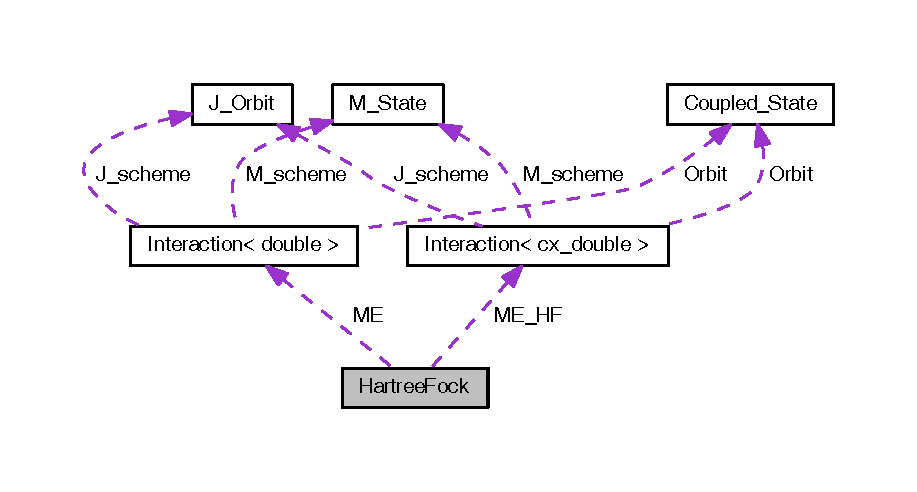
\includegraphics[width=350pt]{class_hartree_fock__coll__graph}
\end{center}
\end{figure}
\subsection*{Public Member Functions}
\begin{DoxyCompactItemize}
\item 
\hyperlink{class_hartree_fock_a0138ea06db729472531ba768af7d0f4f}{Hartree\-Fock} (int Z, int A, string space, string force)
\item 
\hyperlink{class_hartree_fock_a82ad40272840da4287b9a602415beac4}{$\sim$\-Hartree\-Fock} ()
\item 
{\footnotesize template$<$typename T1 , typename T2 $>$ }\\void \hyperlink{class_hartree_fock_a455afd726ee175800c437ac957fab978}{Density\-\_\-\-Matrix} (T1 \&psil, T2 \&psir, cx\-\_\-mat \&rhoij, cx\-\_\-double \&overlap)
\begin{DoxyCompactList}\small\item\em Subroutine to compute rho(i,j) for two S\-D's that are not orthogonal using a matrix representation. \end{DoxyCompactList}\item 
void \hyperlink{class_hartree_fock_a489618a047bfb88057bd50d73d79c2e3}{Mean\-\_\-\-Field} (ivec $\ast$index, vec $\ast$tbme, cx\-\_\-mat $\ast$rhoij, cx\-\_\-mat $\ast$gamma)
\begin{DoxyCompactList}\small\item\em Calculates mean-\/field matrix. \end{DoxyCompactList}\item 
void \hyperlink{class_hartree_fock_af85bdddebed73f27c2b883c2d9e8972e}{Hamiltonian\-\_\-sp} (mat \&e\-\_\-sp, cx\-\_\-mat \&gamma, cx\-\_\-mat \&ham)
\begin{DoxyCompactList}\small\item\em Calculates matrix h=T+\-Gamma. \end{DoxyCompactList}\item 
cx\-\_\-double \hyperlink{class_hartree_fock_accb7866bf87089908210f64157668914}{Hamiltonian} (mat $\ast$e\-\_\-sp, ivec $\ast$index, vec $\ast$tbme, cx\-\_\-mat $\ast$rhoij, cx\-\_\-double $\ast$overlap)
\begin{DoxyCompactList}\small\item\em $<$ psil $|$ H $|$ psir $>$ \end{DoxyCompactList}\item 
void \hyperlink{class_hartree_fock_a78d4a33402c7d999286bdc164cc853b5}{Diagonalization} ()
\begin{DoxyCompactList}\small\item\em Diagonlization single particle Harmiltonian. \end{DoxyCompactList}\item 
void \hyperlink{class_hartree_fock_a727be4c17f68c9ce3cbfcaae6f97e752}{Initialization} ()
\begin{DoxyCompactList}\small\item\em Initialize the H\-F wavefunction. \end{DoxyCompactList}\item 
void \hyperlink{class_hartree_fock_a0ae03c7ead906063143f0047d32f1ee1}{Iteration} ()
\item 
void \hyperlink{class_hartree_fock_a1d8f2d0c9841c8b999fa31758b059214}{Broyden} (cx\-\_\-mat $\ast$m)
\item 
{\footnotesize template$<$typename T1 , typename T2 $>$ }\\void \hyperlink{class_hartree_fock_a6e1d4d4e338a2d55746543a230035121}{Rotation} (double alpha, double beta, double gamma, T1 \&src, T2 \&dest, \hyperlink{class_j___orbit}{J\-\_\-\-Orbit} $\ast$jscheme, \hyperlink{class_m___state}{M\-\_\-\-State} $\ast$mscheme, int dim)
\begin{DoxyCompactList}\small\item\em Rotate a state. \end{DoxyCompactList}\item 
void \hyperlink{class_hartree_fock_af5b3a51f8b65bdda59845648a4865d80}{Space\-\_\-\-Inversion} (cx\-\_\-mat \&src, cx\-\_\-mat \&dest, \hyperlink{class_m___state}{M\-\_\-\-State} $\ast$mscheme)
\begin{DoxyCompactList}\small\item\em Parity projection. \end{DoxyCompactList}\item 
void \hyperlink{class_hartree_fock_a83bfa55f6be64c2b678df42801594e52}{A\-M\-P} (cx\-\_\-mat $\ast$psil, cx\-\_\-mat $\ast$psir, vec \&J, vec \&Parity, cx\-\_\-vec \&H, cx\-\_\-vec \&N)
\begin{DoxyCompactList}\small\item\em Angular momentum projection. \end{DoxyCompactList}\item 
cx\-\_\-double \hyperlink{class_hartree_fock_a19fc02314568b45713933525cf62f11c}{Construct\-\_\-\-M\-E} (ivec \&psil, ivec \&psir)
\item 
void \hyperlink{class_hartree_fock_a14aa8c8c8fff19eb82609abc7fb24958}{H\-W\-\_\-\-Equation\-\_\-\-Hermitian} (cx\-\_\-mat \&A, cx\-\_\-mat \&B, vec \&val, cx\-\_\-mat \&wf)
\item 
void \hyperlink{class_hartree_fock_a36141675bcd557c4241e82b9bf964577}{D\-B\-P} ()
\item 
int \hyperlink{class_hartree_fock_a2cb43d38447325572989595370320706}{pack} (ivec \&config)
\item 
ivec \hyperlink{class_hartree_fock_a65f76efc9fb81e474af5985c52861e0d}{unpack} (int config)
\item 
int \hyperlink{class_hartree_fock_af0c009ecdaf0308740355bc6c2482bc2}{Count\-\_\-\-Particle} (int config)
\end{DoxyCompactItemize}
\subsection*{Private Attributes}
\begin{DoxyCompactItemize}
\item 
\hyperlink{class_interaction}{Interaction}$<$ double $>$ \hyperlink{class_hartree_fock_a4a6514cfef19a943db8cb06b245b2f93}{M\-E}
\item 
\hyperlink{class_interaction}{Interaction}$<$ cx\-\_\-double $>$ \hyperlink{class_hartree_fock_abfd928be86a6d127aff8d8c928d30695}{M\-E\-\_\-\-H\-F}
\item 
int \hyperlink{class_hartree_fock_a18404222b2f400fb9c9985e0b7c7e664}{Mass\-Number} \mbox{[}\hyperlink{class_interaction}{Interaction}$<$ double $>$\-::Iso\-Spin\-\_\-\-Z+1\mbox{]}
\item 
cx\-\_\-mat \hyperlink{class_hartree_fock_a1f460784edc46e9b41d4ea047ef3a3a1}{rho} \mbox{[}\hyperlink{class_interaction}{Interaction}$<$ double $>$\-::Iso\-Spin\-\_\-\-Z\mbox{]}
\item 
cx\-\_\-mat \hyperlink{class_hartree_fock_a7e7361a6e064c9983b0e263f250dd615}{bra} \mbox{[}\hyperlink{class_interaction}{Interaction}$<$ double $>$\-::Iso\-Spin\-\_\-\-Z\mbox{]}
\item 
cx\-\_\-mat \hyperlink{class_hartree_fock_a78ba84d83058ad9c7db287beebb154d4}{ket} \mbox{[}\hyperlink{class_interaction}{Interaction}$<$ double $>$\-::Iso\-Spin\-\_\-\-Z\mbox{]}
\item 
cx\-\_\-mat \hyperlink{class_hartree_fock_a0362bdcdbf5969097be8c03576639e53}{V\-\_\-mf} \mbox{[}\hyperlink{class_interaction}{Interaction}$<$ double $>$\-::Iso\-Spin\-\_\-\-Z\mbox{]}
\item 
cx\-\_\-mat \hyperlink{class_hartree_fock_a4cd7c0aece3eec0c593638763f846d36}{H\-\_\-sp} \mbox{[}\hyperlink{class_interaction}{Interaction}$<$ double $>$\-::Iso\-Spin\-\_\-\-Z\mbox{]}
\item 
vec \hyperlink{class_hartree_fock_a1bb866f2ea89dc0d44f70e1d8e6b1425}{E\-\_\-sp} \mbox{[}\hyperlink{class_interaction}{Interaction}$<$ double $>$\-::Iso\-Spin\-\_\-\-Z\mbox{]}
\item 
double \hyperlink{class_hartree_fock_ae654600f841836c3cb98abee72bf6c35}{B\-E}
\end{DoxyCompactItemize}
\subsection*{Friends}
\begin{DoxyCompactItemize}
\item 
class \hyperlink{class_hartree_fock_a645d83d6370a8adf666416d08c846ddd}{Nucleus}
\end{DoxyCompactItemize}


\subsection{Constructor \& Destructor Documentation}
\hypertarget{class_hartree_fock_a0138ea06db729472531ba768af7d0f4f}{\index{Hartree\-Fock@{Hartree\-Fock}!Hartree\-Fock@{Hartree\-Fock}}
\index{Hartree\-Fock@{Hartree\-Fock}!HartreeFock@{Hartree\-Fock}}
\subsubsection[{Hartree\-Fock}]{\setlength{\rightskip}{0pt plus 5cm}Hartree\-Fock\-::\-Hartree\-Fock (
\begin{DoxyParamCaption}
\item[{int}]{Z, }
\item[{int}]{A, }
\item[{string}]{space, }
\item[{string}]{force}
\end{DoxyParamCaption}
)}}\label{class_hartree_fock_a0138ea06db729472531ba768af7d0f4f}
\hypertarget{class_hartree_fock_a82ad40272840da4287b9a602415beac4}{\index{Hartree\-Fock@{Hartree\-Fock}!$\sim$\-Hartree\-Fock@{$\sim$\-Hartree\-Fock}}
\index{$\sim$\-Hartree\-Fock@{$\sim$\-Hartree\-Fock}!HartreeFock@{Hartree\-Fock}}
\subsubsection[{$\sim$\-Hartree\-Fock}]{\setlength{\rightskip}{0pt plus 5cm}Hartree\-Fock\-::$\sim$\-Hartree\-Fock (
\begin{DoxyParamCaption}
{}
\end{DoxyParamCaption}
)\hspace{0.3cm}{\ttfamily [inline]}}}\label{class_hartree_fock_a82ad40272840da4287b9a602415beac4}


\subsection{Member Function Documentation}
\hypertarget{class_hartree_fock_a83bfa55f6be64c2b678df42801594e52}{\index{Hartree\-Fock@{Hartree\-Fock}!A\-M\-P@{A\-M\-P}}
\index{A\-M\-P@{A\-M\-P}!HartreeFock@{Hartree\-Fock}}
\subsubsection[{A\-M\-P}]{\setlength{\rightskip}{0pt plus 5cm}void Hartree\-Fock\-::\-A\-M\-P (
\begin{DoxyParamCaption}
\item[{cx\-\_\-mat $\ast$}]{psil, }
\item[{cx\-\_\-mat $\ast$}]{psir, }
\item[{vec \&}]{J, }
\item[{vec \&}]{Parity, }
\item[{cx\-\_\-vec \&}]{H, }
\item[{cx\-\_\-vec \&}]{N}
\end{DoxyParamCaption}
)}}\label{class_hartree_fock_a83bfa55f6be64c2b678df42801594e52}


Angular momentum projection. 


\begin{DoxyParams}{Parameters}
{\em Bra\-\_\-\-W\-F} & \\
\hline
{\em Ket\-\_\-\-W\-F} & \\
\hline
{\em J} & angular momentum \\
\hline
{\em P} & parity \\
\hline
\end{DoxyParams}
\begin{DoxyReturn}{Returns}
Hamiltonian 
\end{DoxyReturn}


Here is the call graph for this function\-:
\nopagebreak
\begin{figure}[H]
\begin{center}
\leavevmode
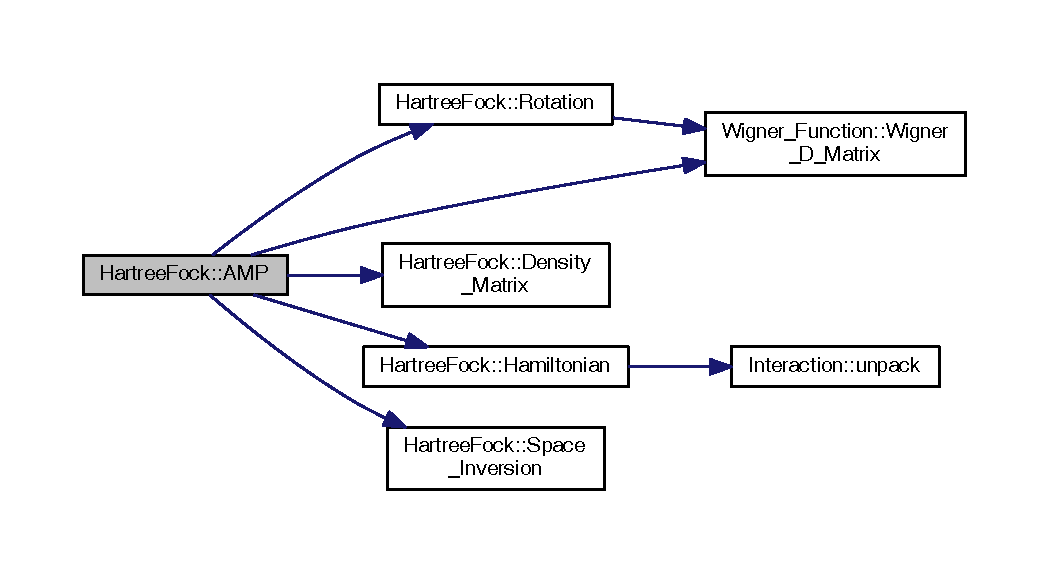
\includegraphics[width=350pt]{class_hartree_fock_a83bfa55f6be64c2b678df42801594e52_cgraph}
\end{center}
\end{figure}




Here is the caller graph for this function\-:
\nopagebreak
\begin{figure}[H]
\begin{center}
\leavevmode
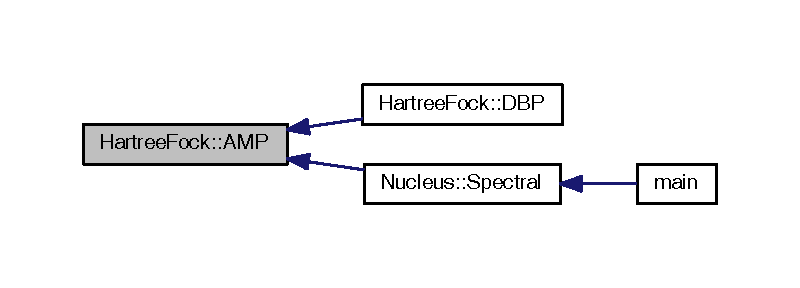
\includegraphics[width=350pt]{class_hartree_fock_a83bfa55f6be64c2b678df42801594e52_icgraph}
\end{center}
\end{figure}


\hypertarget{class_hartree_fock_a1d8f2d0c9841c8b999fa31758b059214}{\index{Hartree\-Fock@{Hartree\-Fock}!Broyden@{Broyden}}
\index{Broyden@{Broyden}!HartreeFock@{Hartree\-Fock}}
\subsubsection[{Broyden}]{\setlength{\rightskip}{0pt plus 5cm}void Hartree\-Fock\-::\-Broyden (
\begin{DoxyParamCaption}
\item[{cx\-\_\-mat $\ast$}]{m}
\end{DoxyParamCaption}
)}}\label{class_hartree_fock_a1d8f2d0c9841c8b999fa31758b059214}


Here is the caller graph for this function\-:
\nopagebreak
\begin{figure}[H]
\begin{center}
\leavevmode
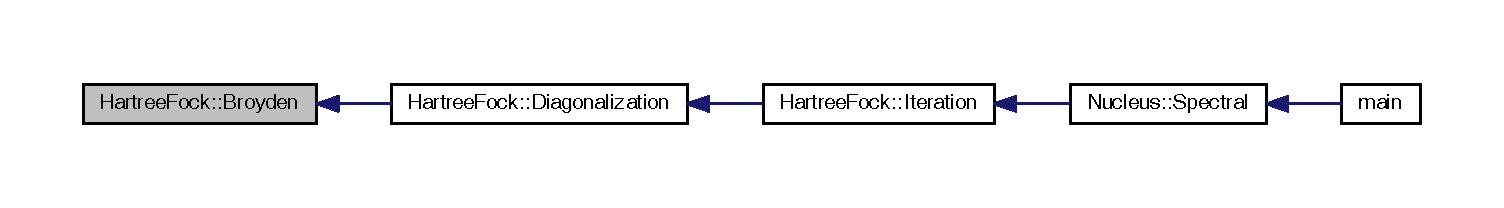
\includegraphics[width=350pt]{class_hartree_fock_a1d8f2d0c9841c8b999fa31758b059214_icgraph}
\end{center}
\end{figure}


\hypertarget{class_hartree_fock_a19fc02314568b45713933525cf62f11c}{\index{Hartree\-Fock@{Hartree\-Fock}!Construct\-\_\-\-M\-E@{Construct\-\_\-\-M\-E}}
\index{Construct\-\_\-\-M\-E@{Construct\-\_\-\-M\-E}!HartreeFock@{Hartree\-Fock}}
\subsubsection[{Construct\-\_\-\-M\-E}]{\setlength{\rightskip}{0pt plus 5cm}cx\-\_\-double Hartree\-Fock\-::\-Construct\-\_\-\-M\-E (
\begin{DoxyParamCaption}
\item[{ivec \&}]{psil, }
\item[{ivec \&}]{psir}
\end{DoxyParamCaption}
)}}\label{class_hartree_fock_a19fc02314568b45713933525cf62f11c}
pp, nn interaction

pn interaction

pp, nn interaction

!!!0.5$\ast$phase$\ast$phase2$\ast$\-M\-E\-\_\-\-H\-F.T\-B\-M\-E\mbox{[}pn\mbox{]}(n);

pn interaction

!!!0.5$\ast$phase$\ast$\-M\-E\-\_\-\-H\-F.T\-B\-M\-E\mbox{[}iso\mbox{]}(n);

pn interaction

!!!0.5$\ast$phase$\ast$\-M\-E\-\_\-\-H\-F.T\-B\-M\-E\mbox{[}iso\mbox{]}(n);

pp, nn interaction

!!!0.5$\ast$phase$\ast$\-M\-E\-\_\-\-H\-F.T\-B\-M\-E\mbox{[}pn\mbox{]}(n); 

Here is the call graph for this function\-:
\nopagebreak
\begin{figure}[H]
\begin{center}
\leavevmode
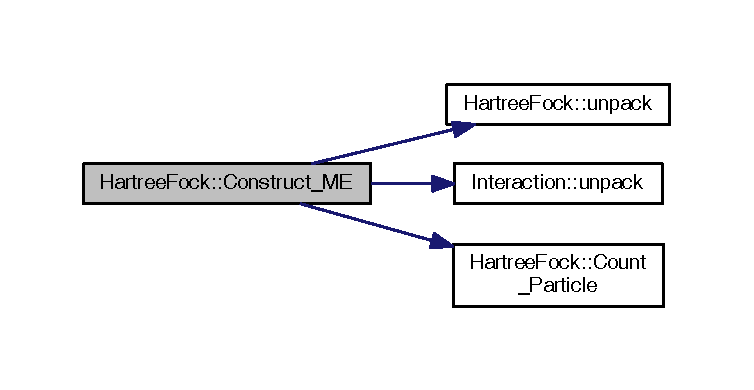
\includegraphics[width=350pt]{class_hartree_fock_a19fc02314568b45713933525cf62f11c_cgraph}
\end{center}
\end{figure}




Here is the caller graph for this function\-:
\nopagebreak
\begin{figure}[H]
\begin{center}
\leavevmode
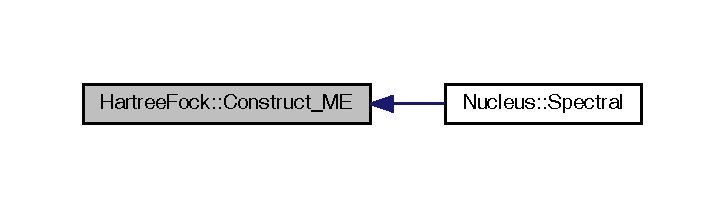
\includegraphics[width=348pt]{class_hartree_fock_a19fc02314568b45713933525cf62f11c_icgraph}
\end{center}
\end{figure}


\hypertarget{class_hartree_fock_af0c009ecdaf0308740355bc6c2482bc2}{\index{Hartree\-Fock@{Hartree\-Fock}!Count\-\_\-\-Particle@{Count\-\_\-\-Particle}}
\index{Count\-\_\-\-Particle@{Count\-\_\-\-Particle}!HartreeFock@{Hartree\-Fock}}
\subsubsection[{Count\-\_\-\-Particle}]{\setlength{\rightskip}{0pt plus 5cm}int Hartree\-Fock\-::\-Count\-\_\-\-Particle (
\begin{DoxyParamCaption}
\item[{int}]{config}
\end{DoxyParamCaption}
)}}\label{class_hartree_fock_af0c009ecdaf0308740355bc6c2482bc2}


Here is the caller graph for this function\-:
\nopagebreak
\begin{figure}[H]
\begin{center}
\leavevmode
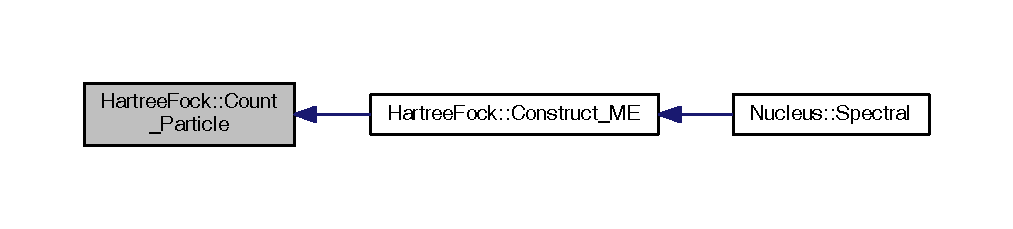
\includegraphics[width=350pt]{class_hartree_fock_af0c009ecdaf0308740355bc6c2482bc2_icgraph}
\end{center}
\end{figure}


\hypertarget{class_hartree_fock_a36141675bcd557c4241e82b9bf964577}{\index{Hartree\-Fock@{Hartree\-Fock}!D\-B\-P@{D\-B\-P}}
\index{D\-B\-P@{D\-B\-P}!HartreeFock@{Hartree\-Fock}}
\subsubsection[{D\-B\-P}]{\setlength{\rightskip}{0pt plus 5cm}void Hartree\-Fock\-::\-D\-B\-P (
\begin{DoxyParamCaption}
{}
\end{DoxyParamCaption}
)}}\label{class_hartree_fock_a36141675bcd557c4241e82b9bf964577}


Here is the call graph for this function\-:
\nopagebreak
\begin{figure}[H]
\begin{center}
\leavevmode
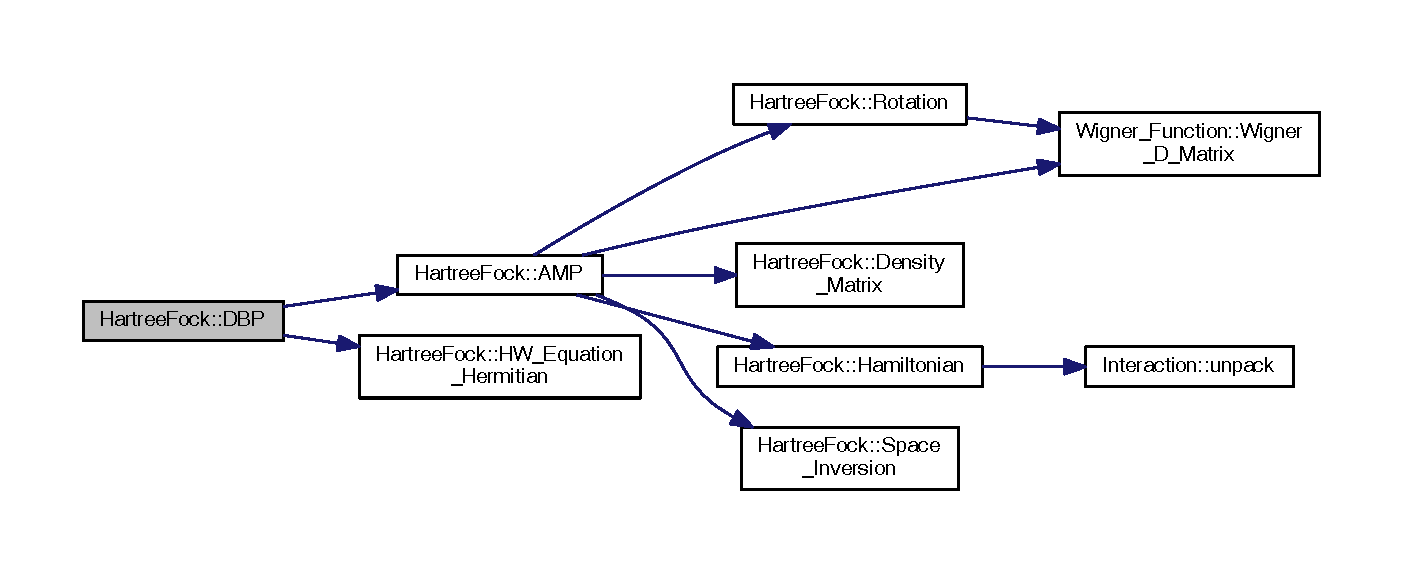
\includegraphics[width=350pt]{class_hartree_fock_a36141675bcd557c4241e82b9bf964577_cgraph}
\end{center}
\end{figure}


\hypertarget{class_hartree_fock_a455afd726ee175800c437ac957fab978}{\index{Hartree\-Fock@{Hartree\-Fock}!Density\-\_\-\-Matrix@{Density\-\_\-\-Matrix}}
\index{Density\-\_\-\-Matrix@{Density\-\_\-\-Matrix}!HartreeFock@{Hartree\-Fock}}
\subsubsection[{Density\-\_\-\-Matrix}]{\setlength{\rightskip}{0pt plus 5cm}template$<$typename T1 , typename T2 $>$ void Hartree\-Fock\-::\-Density\-\_\-\-Matrix (
\begin{DoxyParamCaption}
\item[{T1 \&}]{psil, }
\item[{T2 \&}]{psir, }
\item[{cx\-\_\-mat \&}]{rhoij, }
\item[{cx\-\_\-double \&}]{overlap}
\end{DoxyParamCaption}
)}}\label{class_hartree_fock_a455afd726ee175800c437ac957fab978}


Subroutine to compute rho(i,j) for two S\-D's that are not orthogonal using a matrix representation. 


\begin{DoxyParams}{Parameters}
{\em psir} & right S\-D \\
\hline
{\em psil} & left S\-D \\
\hline
\end{DoxyParams}
\begin{DoxyReturn}{Returns}
rhoij\-: density matrix $<$ psil $|$ a$^\wedge$ a\-\_\-j $|$ psir $>$ 

overlap\-: $<$ psil $|$ psir $>$ 
\end{DoxyReturn}
!!!!!! S\-V\-D may be more suitable 

Here is the caller graph for this function\-:
\nopagebreak
\begin{figure}[H]
\begin{center}
\leavevmode
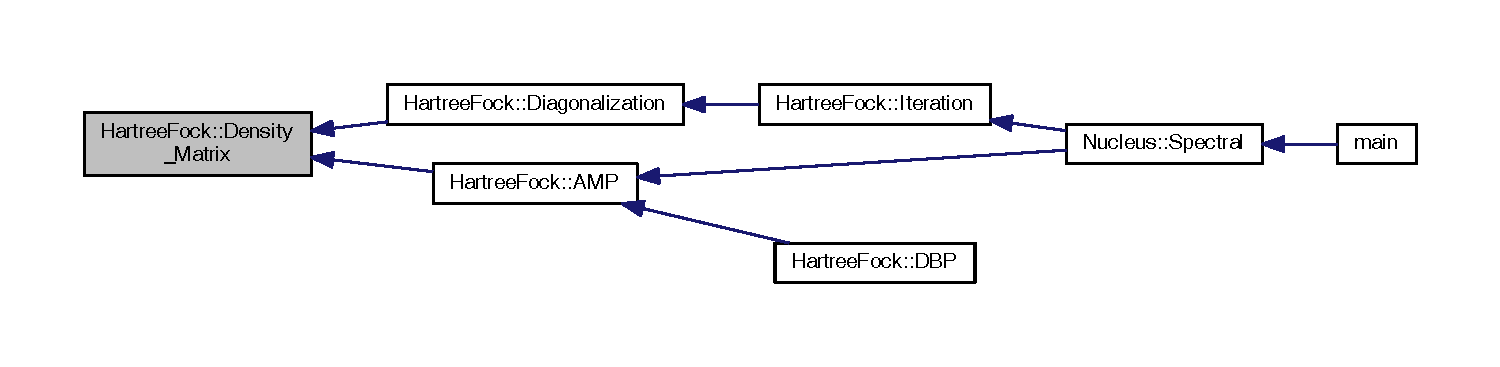
\includegraphics[width=350pt]{class_hartree_fock_a455afd726ee175800c437ac957fab978_icgraph}
\end{center}
\end{figure}


\hypertarget{class_hartree_fock_a78d4a33402c7d999286bdc164cc853b5}{\index{Hartree\-Fock@{Hartree\-Fock}!Diagonalization@{Diagonalization}}
\index{Diagonalization@{Diagonalization}!HartreeFock@{Hartree\-Fock}}
\subsubsection[{Diagonalization}]{\setlength{\rightskip}{0pt plus 5cm}void Hartree\-Fock\-::\-Diagonalization (
\begin{DoxyParamCaption}
{}
\end{DoxyParamCaption}
)}}\label{class_hartree_fock_a78d4a33402c7d999286bdc164cc853b5}


Diagonlization single particle Harmiltonian. 


\begin{DoxyParams}{Parameters}
{\em Hamiltonian\-\_\-sp} & \\
\hline
\end{DoxyParams}
\begin{DoxyReturn}{Returns}
Energies 

Wavefunctions 
\end{DoxyReturn}


Here is the call graph for this function\-:
\nopagebreak
\begin{figure}[H]
\begin{center}
\leavevmode
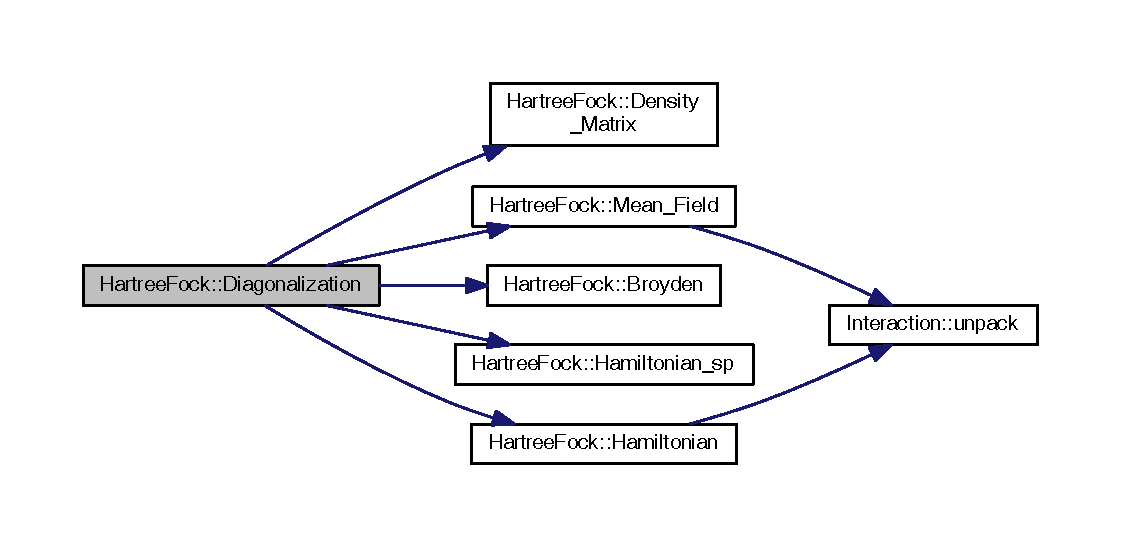
\includegraphics[width=350pt]{class_hartree_fock_a78d4a33402c7d999286bdc164cc853b5_cgraph}
\end{center}
\end{figure}




Here is the caller graph for this function\-:
\nopagebreak
\begin{figure}[H]
\begin{center}
\leavevmode
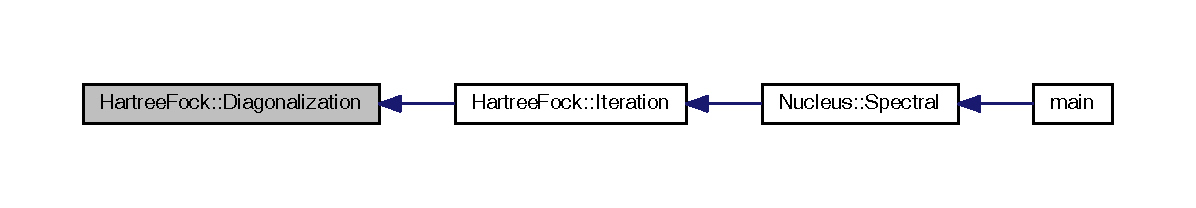
\includegraphics[width=350pt]{class_hartree_fock_a78d4a33402c7d999286bdc164cc853b5_icgraph}
\end{center}
\end{figure}


\hypertarget{class_hartree_fock_accb7866bf87089908210f64157668914}{\index{Hartree\-Fock@{Hartree\-Fock}!Hamiltonian@{Hamiltonian}}
\index{Hamiltonian@{Hamiltonian}!HartreeFock@{Hartree\-Fock}}
\subsubsection[{Hamiltonian}]{\setlength{\rightskip}{0pt plus 5cm}cx\-\_\-double Hartree\-Fock\-::\-Hamiltonian (
\begin{DoxyParamCaption}
\item[{mat $\ast$}]{e\-\_\-sp, }
\item[{ivec $\ast$}]{index, }
\item[{vec $\ast$}]{tbme, }
\item[{cx\-\_\-mat $\ast$}]{rhoij, }
\item[{cx\-\_\-double $\ast$}]{overlap}
\end{DoxyParamCaption}
)}}\label{class_hartree_fock_accb7866bf87089908210f64157668914}


$<$ psil $|$ H $|$ psir $>$ 


\begin{DoxyParams}{Parameters}
{\em e\-\_\-sp(i,j)} & one-\/body matrix element between i,j m-\/states \\
\hline
{\em Index(i)} & list of (packed) nonzero indices, i = 1 to nmatpp to get indices I\-J\-K\-L of i'th matrix element do U\-N\-P\-A\-C\-K(\-Index) \\
\hline
{\em T\-B\-M\-E(i)} & ith T\-B\-M\-E associated with indices unpacked from Index(i) \\
\hline
\end{DoxyParams}
\begin{DoxyReturn}{Returns}
rhoij density matrix $<$ psil $|$ a$^\wedge$ a\-\_\-j $|$ psir $>$ 

$<$ psil $|$ H $|$ psir $>$ 
\end{DoxyReturn}
O\-B\-M\-E

pp, nn interaction

pn interaction 

Here is the call graph for this function\-:
\nopagebreak
\begin{figure}[H]
\begin{center}
\leavevmode
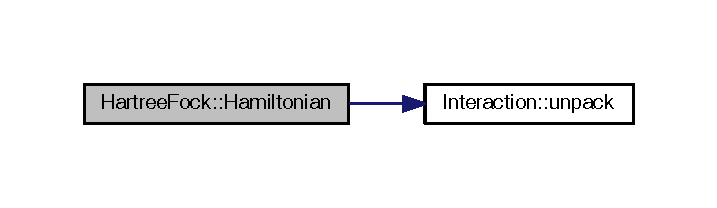
\includegraphics[width=344pt]{class_hartree_fock_accb7866bf87089908210f64157668914_cgraph}
\end{center}
\end{figure}




Here is the caller graph for this function\-:
\nopagebreak
\begin{figure}[H]
\begin{center}
\leavevmode
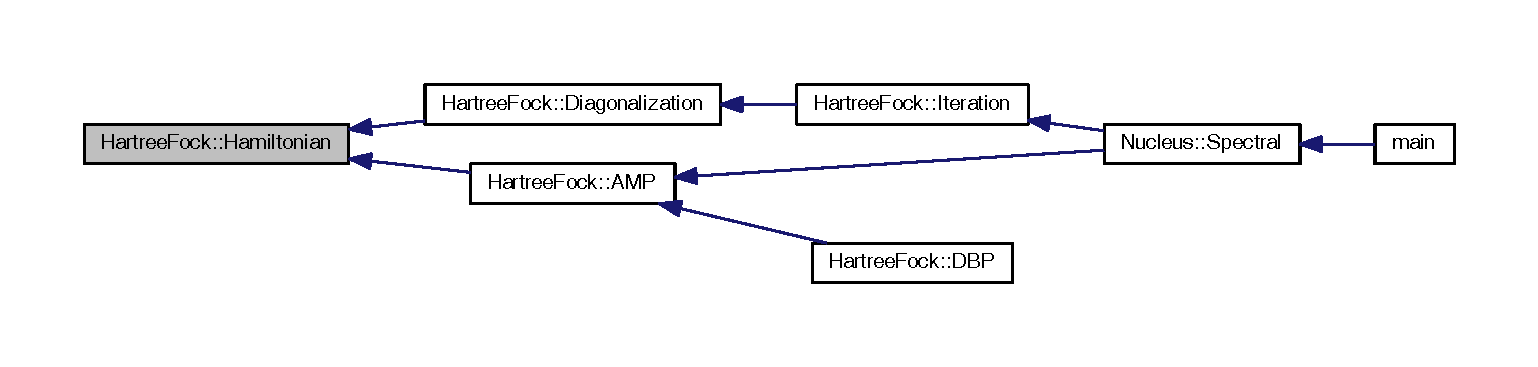
\includegraphics[width=350pt]{class_hartree_fock_accb7866bf87089908210f64157668914_icgraph}
\end{center}
\end{figure}


\hypertarget{class_hartree_fock_af85bdddebed73f27c2b883c2d9e8972e}{\index{Hartree\-Fock@{Hartree\-Fock}!Hamiltonian\-\_\-sp@{Hamiltonian\-\_\-sp}}
\index{Hamiltonian\-\_\-sp@{Hamiltonian\-\_\-sp}!HartreeFock@{Hartree\-Fock}}
\subsubsection[{Hamiltonian\-\_\-sp}]{\setlength{\rightskip}{0pt plus 5cm}void Hartree\-Fock\-::\-Hamiltonian\-\_\-sp (
\begin{DoxyParamCaption}
\item[{mat \&}]{e\-\_\-sp, }
\item[{cx\-\_\-mat \&}]{gamma, }
\item[{cx\-\_\-mat \&}]{ham}
\end{DoxyParamCaption}
)}}\label{class_hartree_fock_af85bdddebed73f27c2b883c2d9e8972e}


Calculates matrix h=T+\-Gamma. 


\begin{DoxyParams}{Parameters}
{\em e\-\_\-sp(i,j)} & one-\/body matrix element between i,j m-\/states \\
\hline
{\em gamma} & Gamma matrix \\
\hline
\end{DoxyParams}
\begin{DoxyReturn}{Returns}
Hamiltonian\-\_\-sp 
\end{DoxyReturn}


Here is the caller graph for this function\-:
\nopagebreak
\begin{figure}[H]
\begin{center}
\leavevmode
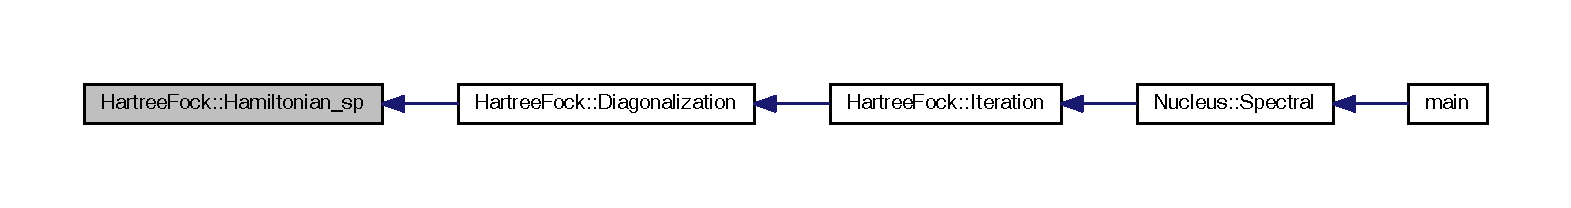
\includegraphics[width=350pt]{class_hartree_fock_af85bdddebed73f27c2b883c2d9e8972e_icgraph}
\end{center}
\end{figure}


\hypertarget{class_hartree_fock_a14aa8c8c8fff19eb82609abc7fb24958}{\index{Hartree\-Fock@{Hartree\-Fock}!H\-W\-\_\-\-Equation\-\_\-\-Hermitian@{H\-W\-\_\-\-Equation\-\_\-\-Hermitian}}
\index{H\-W\-\_\-\-Equation\-\_\-\-Hermitian@{H\-W\-\_\-\-Equation\-\_\-\-Hermitian}!HartreeFock@{Hartree\-Fock}}
\subsubsection[{H\-W\-\_\-\-Equation\-\_\-\-Hermitian}]{\setlength{\rightskip}{0pt plus 5cm}void Hartree\-Fock\-::\-H\-W\-\_\-\-Equation\-\_\-\-Hermitian (
\begin{DoxyParamCaption}
\item[{cx\-\_\-mat \&}]{A, }
\item[{cx\-\_\-mat \&}]{B, }
\item[{vec \&}]{val, }
\item[{cx\-\_\-mat \&}]{wf}
\end{DoxyParamCaption}
)}}\label{class_hartree_fock_a14aa8c8c8fff19eb82609abc7fb24958}


Here is the caller graph for this function\-:
\nopagebreak
\begin{figure}[H]
\begin{center}
\leavevmode
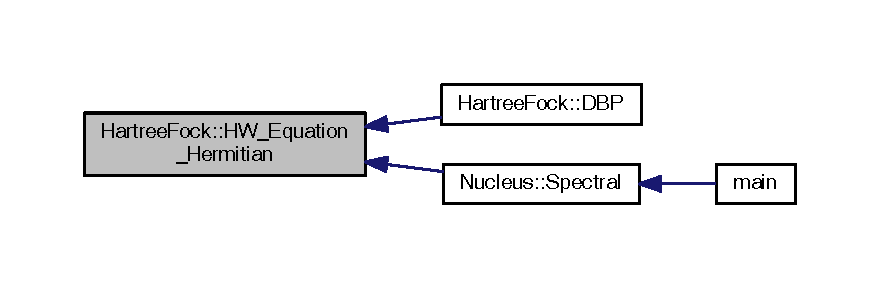
\includegraphics[width=350pt]{class_hartree_fock_a14aa8c8c8fff19eb82609abc7fb24958_icgraph}
\end{center}
\end{figure}


\hypertarget{class_hartree_fock_a727be4c17f68c9ce3cbfcaae6f97e752}{\index{Hartree\-Fock@{Hartree\-Fock}!Initialization@{Initialization}}
\index{Initialization@{Initialization}!HartreeFock@{Hartree\-Fock}}
\subsubsection[{Initialization}]{\setlength{\rightskip}{0pt plus 5cm}void Hartree\-Fock\-::\-Initialization (
\begin{DoxyParamCaption}
{}
\end{DoxyParamCaption}
)}}\label{class_hartree_fock_a727be4c17f68c9ce3cbfcaae6f97e752}


Initialize the H\-F wavefunction. 

\begin{DoxyReturn}{Returns}
Bra\-\_\-\-W\-F 

Ket\-\_\-\-W\-F 
\end{DoxyReturn}


Here is the caller graph for this function\-:
\nopagebreak
\begin{figure}[H]
\begin{center}
\leavevmode
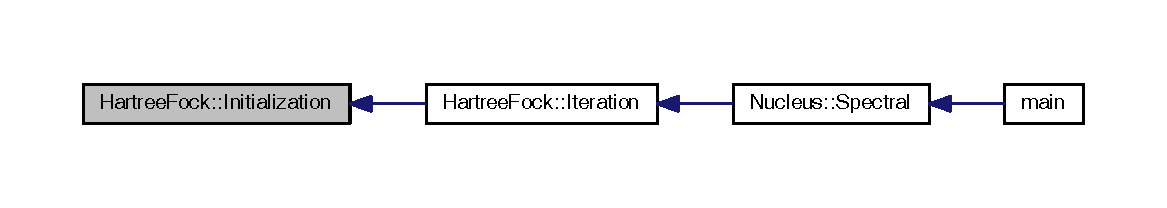
\includegraphics[width=350pt]{class_hartree_fock_a727be4c17f68c9ce3cbfcaae6f97e752_icgraph}
\end{center}
\end{figure}


\hypertarget{class_hartree_fock_a0ae03c7ead906063143f0047d32f1ee1}{\index{Hartree\-Fock@{Hartree\-Fock}!Iteration@{Iteration}}
\index{Iteration@{Iteration}!HartreeFock@{Hartree\-Fock}}
\subsubsection[{Iteration}]{\setlength{\rightskip}{0pt plus 5cm}void Hartree\-Fock\-::\-Iteration (
\begin{DoxyParamCaption}
{}
\end{DoxyParamCaption}
)}}\label{class_hartree_fock_a0ae03c7ead906063143f0047d32f1ee1}


Here is the call graph for this function\-:
\nopagebreak
\begin{figure}[H]
\begin{center}
\leavevmode
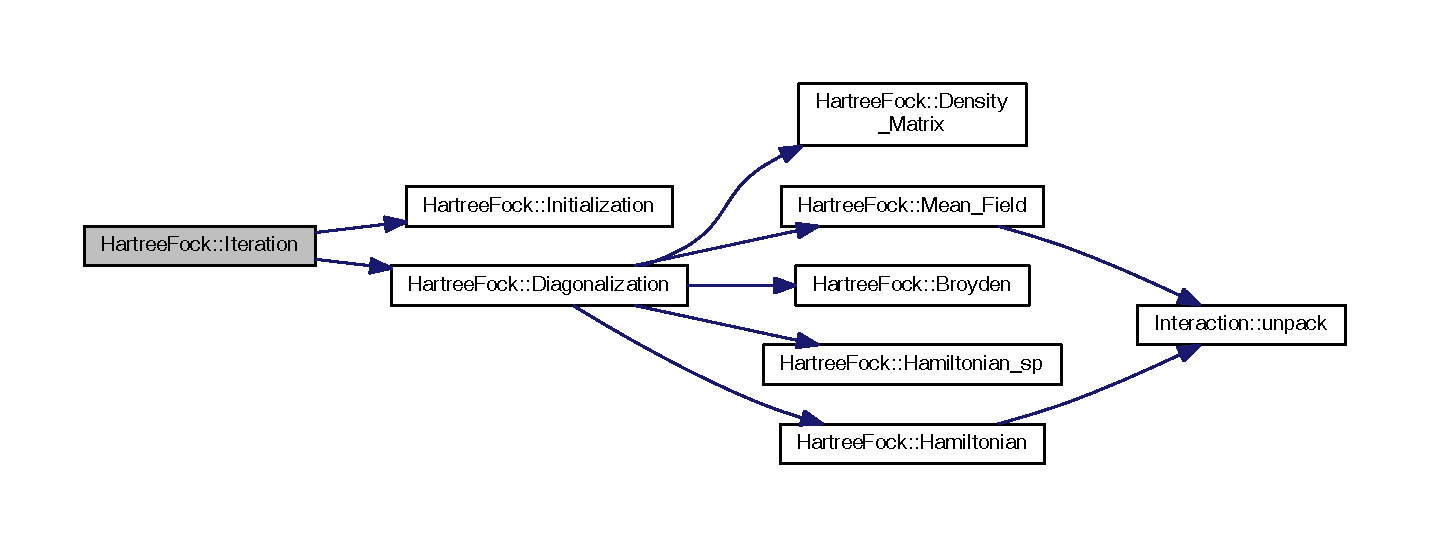
\includegraphics[width=350pt]{class_hartree_fock_a0ae03c7ead906063143f0047d32f1ee1_cgraph}
\end{center}
\end{figure}




Here is the caller graph for this function\-:
\nopagebreak
\begin{figure}[H]
\begin{center}
\leavevmode
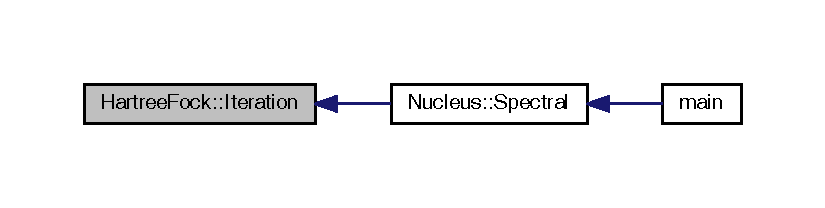
\includegraphics[width=350pt]{class_hartree_fock_a0ae03c7ead906063143f0047d32f1ee1_icgraph}
\end{center}
\end{figure}


\hypertarget{class_hartree_fock_a489618a047bfb88057bd50d73d79c2e3}{\index{Hartree\-Fock@{Hartree\-Fock}!Mean\-\_\-\-Field@{Mean\-\_\-\-Field}}
\index{Mean\-\_\-\-Field@{Mean\-\_\-\-Field}!HartreeFock@{Hartree\-Fock}}
\subsubsection[{Mean\-\_\-\-Field}]{\setlength{\rightskip}{0pt plus 5cm}void Hartree\-Fock\-::\-Mean\-\_\-\-Field (
\begin{DoxyParamCaption}
\item[{ivec $\ast$}]{index, }
\item[{vec $\ast$}]{tbme, }
\item[{cx\-\_\-mat $\ast$}]{rhoij, }
\item[{cx\-\_\-mat $\ast$}]{gamma}
\end{DoxyParamCaption}
)}}\label{class_hartree_fock_a489618a047bfb88057bd50d73d79c2e3}


Calculates mean-\/field matrix. 


\begin{DoxyParams}{Parameters}
{\em Index(i)} & list of (packed) nonzero indices, i = 1 to nmatpp to get indices I\-J\-K\-L of i'th matrix element do U\-N\-P\-A\-C\-K(\-Index) \\
\hline
{\em T\-B\-M\-E(i)} & ith T\-B\-M\-E associated with indices unpacked from Index(i) \\
\hline
{\em rhopij/rhonij} & density matices for protons/neutrons \\
\hline
\end{DoxyParams}
\begin{DoxyReturn}{Returns}
gammap/gamman\-: Gamma matrix for protons/neutrons 
\end{DoxyReturn}


Here is the call graph for this function\-:
\nopagebreak
\begin{figure}[H]
\begin{center}
\leavevmode
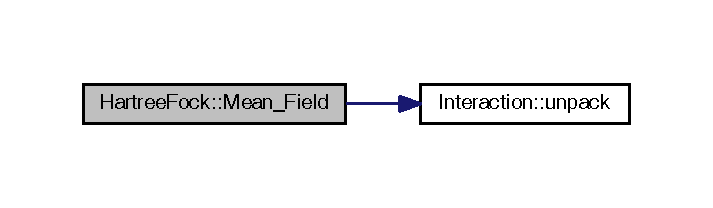
\includegraphics[width=342pt]{class_hartree_fock_a489618a047bfb88057bd50d73d79c2e3_cgraph}
\end{center}
\end{figure}




Here is the caller graph for this function\-:
\nopagebreak
\begin{figure}[H]
\begin{center}
\leavevmode
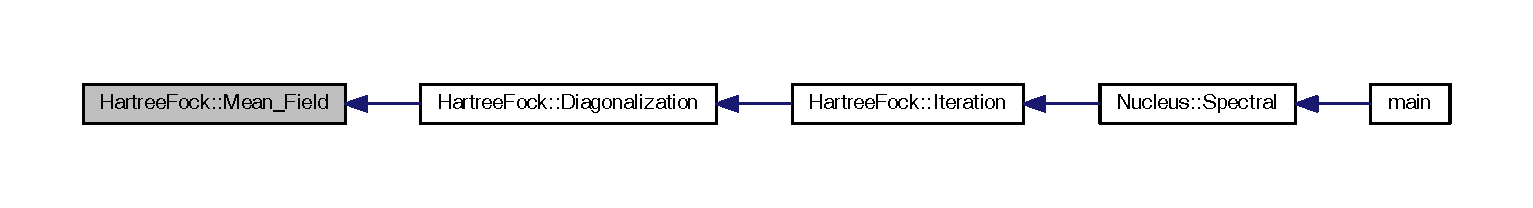
\includegraphics[width=350pt]{class_hartree_fock_a489618a047bfb88057bd50d73d79c2e3_icgraph}
\end{center}
\end{figure}


\hypertarget{class_hartree_fock_a2cb43d38447325572989595370320706}{\index{Hartree\-Fock@{Hartree\-Fock}!pack@{pack}}
\index{pack@{pack}!HartreeFock@{Hartree\-Fock}}
\subsubsection[{pack}]{\setlength{\rightskip}{0pt plus 5cm}int Hartree\-Fock\-::pack (
\begin{DoxyParamCaption}
\item[{ivec \&}]{config}
\end{DoxyParamCaption}
)}}\label{class_hartree_fock_a2cb43d38447325572989595370320706}


Here is the caller graph for this function\-:
\nopagebreak
\begin{figure}[H]
\begin{center}
\leavevmode
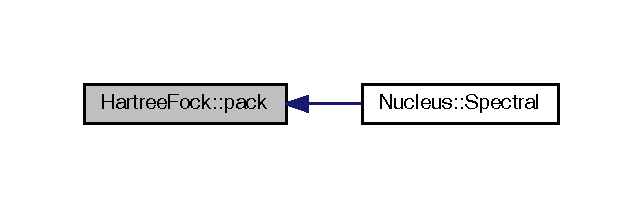
\includegraphics[width=308pt]{class_hartree_fock_a2cb43d38447325572989595370320706_icgraph}
\end{center}
\end{figure}


\hypertarget{class_hartree_fock_a6e1d4d4e338a2d55746543a230035121}{\index{Hartree\-Fock@{Hartree\-Fock}!Rotation@{Rotation}}
\index{Rotation@{Rotation}!HartreeFock@{Hartree\-Fock}}
\subsubsection[{Rotation}]{\setlength{\rightskip}{0pt plus 5cm}template$<$typename T1 , typename T2 $>$ void Hartree\-Fock\-::\-Rotation (
\begin{DoxyParamCaption}
\item[{double}]{alpha, }
\item[{double}]{beta, }
\item[{double}]{gamma, }
\item[{T1 \&}]{src, }
\item[{T2 \&}]{dest, }
\item[{{\bf J\-\_\-\-Orbit} $\ast$}]{jscheme, }
\item[{{\bf M\-\_\-\-State} $\ast$}]{mscheme, }
\item[{int}]{dim}
\end{DoxyParamCaption}
)}}\label{class_hartree_fock_a6e1d4d4e338a2d55746543a230035121}


Rotate a state. 


\begin{DoxyParams}{Parameters}
{\em Wavefunction} & \\
\hline
\end{DoxyParams}
\begin{DoxyReturn}{Returns}
Rotated Wavefunction 
\end{DoxyReturn}


Here is the call graph for this function\-:
\nopagebreak
\begin{figure}[H]
\begin{center}
\leavevmode
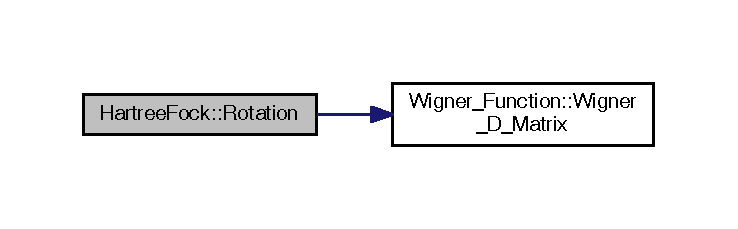
\includegraphics[width=350pt]{class_hartree_fock_a6e1d4d4e338a2d55746543a230035121_cgraph}
\end{center}
\end{figure}




Here is the caller graph for this function\-:
\nopagebreak
\begin{figure}[H]
\begin{center}
\leavevmode
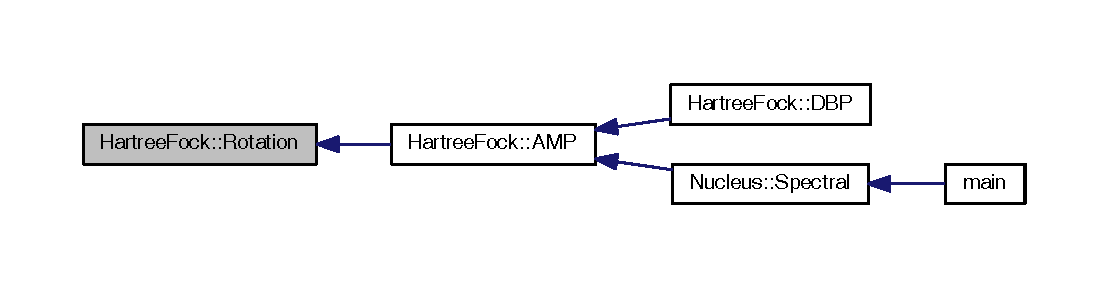
\includegraphics[width=350pt]{class_hartree_fock_a6e1d4d4e338a2d55746543a230035121_icgraph}
\end{center}
\end{figure}


\hypertarget{class_hartree_fock_af5b3a51f8b65bdda59845648a4865d80}{\index{Hartree\-Fock@{Hartree\-Fock}!Space\-\_\-\-Inversion@{Space\-\_\-\-Inversion}}
\index{Space\-\_\-\-Inversion@{Space\-\_\-\-Inversion}!HartreeFock@{Hartree\-Fock}}
\subsubsection[{Space\-\_\-\-Inversion}]{\setlength{\rightskip}{0pt plus 5cm}void Hartree\-Fock\-::\-Space\-\_\-\-Inversion (
\begin{DoxyParamCaption}
\item[{cx\-\_\-mat \&}]{src, }
\item[{cx\-\_\-mat \&}]{dest, }
\item[{{\bf M\-\_\-\-State} $\ast$}]{mscheme}
\end{DoxyParamCaption}
)}}\label{class_hartree_fock_af5b3a51f8b65bdda59845648a4865d80}


Parity projection. 


\begin{DoxyParams}{Parameters}
{\em Wavefunction} & \\
\hline
\end{DoxyParams}
\begin{DoxyReturn}{Returns}
Wavefunction with space inversed 
\end{DoxyReturn}


Here is the caller graph for this function\-:
\nopagebreak
\begin{figure}[H]
\begin{center}
\leavevmode
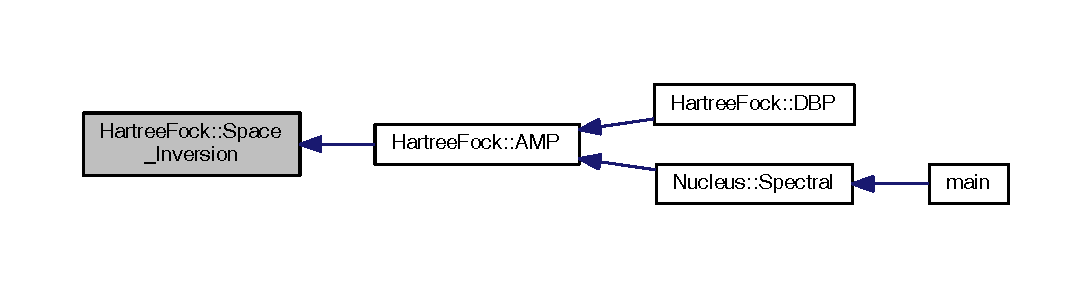
\includegraphics[width=350pt]{class_hartree_fock_af5b3a51f8b65bdda59845648a4865d80_icgraph}
\end{center}
\end{figure}


\hypertarget{class_hartree_fock_a65f76efc9fb81e474af5985c52861e0d}{\index{Hartree\-Fock@{Hartree\-Fock}!unpack@{unpack}}
\index{unpack@{unpack}!HartreeFock@{Hartree\-Fock}}
\subsubsection[{unpack}]{\setlength{\rightskip}{0pt plus 5cm}ivec Hartree\-Fock\-::unpack (
\begin{DoxyParamCaption}
\item[{int}]{config}
\end{DoxyParamCaption}
)}}\label{class_hartree_fock_a65f76efc9fb81e474af5985c52861e0d}


Here is the caller graph for this function\-:
\nopagebreak
\begin{figure}[H]
\begin{center}
\leavevmode
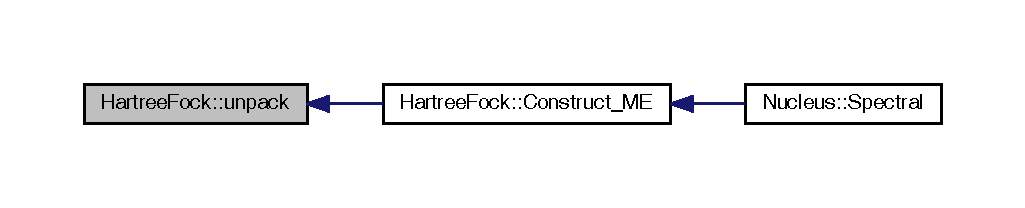
\includegraphics[width=350pt]{class_hartree_fock_a65f76efc9fb81e474af5985c52861e0d_icgraph}
\end{center}
\end{figure}




\subsection{Friends And Related Function Documentation}
\hypertarget{class_hartree_fock_a645d83d6370a8adf666416d08c846ddd}{\index{Hartree\-Fock@{Hartree\-Fock}!Nucleus@{Nucleus}}
\index{Nucleus@{Nucleus}!HartreeFock@{Hartree\-Fock}}
\subsubsection[{Nucleus}]{\setlength{\rightskip}{0pt plus 5cm}friend class {\bf Nucleus}\hspace{0.3cm}{\ttfamily [friend]}}}\label{class_hartree_fock_a645d83d6370a8adf666416d08c846ddd}


\subsection{Member Data Documentation}
\hypertarget{class_hartree_fock_ae654600f841836c3cb98abee72bf6c35}{\index{Hartree\-Fock@{Hartree\-Fock}!B\-E@{B\-E}}
\index{B\-E@{B\-E}!HartreeFock@{Hartree\-Fock}}
\subsubsection[{B\-E}]{\setlength{\rightskip}{0pt plus 5cm}double Hartree\-Fock\-::\-B\-E\hspace{0.3cm}{\ttfamily [private]}}}\label{class_hartree_fock_ae654600f841836c3cb98abee72bf6c35}
\hypertarget{class_hartree_fock_a7e7361a6e064c9983b0e263f250dd615}{\index{Hartree\-Fock@{Hartree\-Fock}!bra@{bra}}
\index{bra@{bra}!HartreeFock@{Hartree\-Fock}}
\subsubsection[{bra}]{\setlength{\rightskip}{0pt plus 5cm}cx\-\_\-mat Hartree\-Fock\-::bra\mbox{[}{\bf Interaction}$<$ double $>$\-::Iso\-Spin\-\_\-\-Z\mbox{]}\hspace{0.3cm}{\ttfamily [private]}}}\label{class_hartree_fock_a7e7361a6e064c9983b0e263f250dd615}
\hypertarget{class_hartree_fock_a1bb866f2ea89dc0d44f70e1d8e6b1425}{\index{Hartree\-Fock@{Hartree\-Fock}!E\-\_\-sp@{E\-\_\-sp}}
\index{E\-\_\-sp@{E\-\_\-sp}!HartreeFock@{Hartree\-Fock}}
\subsubsection[{E\-\_\-sp}]{\setlength{\rightskip}{0pt plus 5cm}vec Hartree\-Fock\-::\-E\-\_\-sp\mbox{[}{\bf Interaction}$<$ double $>$\-::Iso\-Spin\-\_\-\-Z\mbox{]}\hspace{0.3cm}{\ttfamily [private]}}}\label{class_hartree_fock_a1bb866f2ea89dc0d44f70e1d8e6b1425}
\hypertarget{class_hartree_fock_a4cd7c0aece3eec0c593638763f846d36}{\index{Hartree\-Fock@{Hartree\-Fock}!H\-\_\-sp@{H\-\_\-sp}}
\index{H\-\_\-sp@{H\-\_\-sp}!HartreeFock@{Hartree\-Fock}}
\subsubsection[{H\-\_\-sp}]{\setlength{\rightskip}{0pt plus 5cm}cx\-\_\-mat Hartree\-Fock\-::\-H\-\_\-sp\mbox{[}{\bf Interaction}$<$ double $>$\-::Iso\-Spin\-\_\-\-Z\mbox{]}\hspace{0.3cm}{\ttfamily [private]}}}\label{class_hartree_fock_a4cd7c0aece3eec0c593638763f846d36}
\hypertarget{class_hartree_fock_a78ba84d83058ad9c7db287beebb154d4}{\index{Hartree\-Fock@{Hartree\-Fock}!ket@{ket}}
\index{ket@{ket}!HartreeFock@{Hartree\-Fock}}
\subsubsection[{ket}]{\setlength{\rightskip}{0pt plus 5cm}cx\-\_\-mat Hartree\-Fock\-::ket\mbox{[}{\bf Interaction}$<$ double $>$\-::Iso\-Spin\-\_\-\-Z\mbox{]}\hspace{0.3cm}{\ttfamily [private]}}}\label{class_hartree_fock_a78ba84d83058ad9c7db287beebb154d4}
\hypertarget{class_hartree_fock_a18404222b2f400fb9c9985e0b7c7e664}{\index{Hartree\-Fock@{Hartree\-Fock}!Mass\-Number@{Mass\-Number}}
\index{Mass\-Number@{Mass\-Number}!HartreeFock@{Hartree\-Fock}}
\subsubsection[{Mass\-Number}]{\setlength{\rightskip}{0pt plus 5cm}int Hartree\-Fock\-::\-Mass\-Number\mbox{[}{\bf Interaction}$<$ double $>$\-::Iso\-Spin\-\_\-\-Z+1\mbox{]}\hspace{0.3cm}{\ttfamily [private]}}}\label{class_hartree_fock_a18404222b2f400fb9c9985e0b7c7e664}
\hypertarget{class_hartree_fock_a4a6514cfef19a943db8cb06b245b2f93}{\index{Hartree\-Fock@{Hartree\-Fock}!M\-E@{M\-E}}
\index{M\-E@{M\-E}!HartreeFock@{Hartree\-Fock}}
\subsubsection[{M\-E}]{\setlength{\rightskip}{0pt plus 5cm}{\bf Interaction}$<$double$>$ Hartree\-Fock\-::\-M\-E\hspace{0.3cm}{\ttfamily [private]}}}\label{class_hartree_fock_a4a6514cfef19a943db8cb06b245b2f93}
\hypertarget{class_hartree_fock_abfd928be86a6d127aff8d8c928d30695}{\index{Hartree\-Fock@{Hartree\-Fock}!M\-E\-\_\-\-H\-F@{M\-E\-\_\-\-H\-F}}
\index{M\-E\-\_\-\-H\-F@{M\-E\-\_\-\-H\-F}!HartreeFock@{Hartree\-Fock}}
\subsubsection[{M\-E\-\_\-\-H\-F}]{\setlength{\rightskip}{0pt plus 5cm}{\bf Interaction}$<$cx\-\_\-double$>$ Hartree\-Fock\-::\-M\-E\-\_\-\-H\-F\hspace{0.3cm}{\ttfamily [private]}}}\label{class_hartree_fock_abfd928be86a6d127aff8d8c928d30695}
\hypertarget{class_hartree_fock_a1f460784edc46e9b41d4ea047ef3a3a1}{\index{Hartree\-Fock@{Hartree\-Fock}!rho@{rho}}
\index{rho@{rho}!HartreeFock@{Hartree\-Fock}}
\subsubsection[{rho}]{\setlength{\rightskip}{0pt plus 5cm}cx\-\_\-mat Hartree\-Fock\-::rho\mbox{[}{\bf Interaction}$<$ double $>$\-::Iso\-Spin\-\_\-\-Z\mbox{]}\hspace{0.3cm}{\ttfamily [private]}}}\label{class_hartree_fock_a1f460784edc46e9b41d4ea047ef3a3a1}
\hypertarget{class_hartree_fock_a0362bdcdbf5969097be8c03576639e53}{\index{Hartree\-Fock@{Hartree\-Fock}!V\-\_\-mf@{V\-\_\-mf}}
\index{V\-\_\-mf@{V\-\_\-mf}!HartreeFock@{Hartree\-Fock}}
\subsubsection[{V\-\_\-mf}]{\setlength{\rightskip}{0pt plus 5cm}cx\-\_\-mat Hartree\-Fock\-::\-V\-\_\-mf\mbox{[}{\bf Interaction}$<$ double $>$\-::Iso\-Spin\-\_\-\-Z\mbox{]}\hspace{0.3cm}{\ttfamily [private]}}}\label{class_hartree_fock_a0362bdcdbf5969097be8c03576639e53}


The documentation for this class was generated from the following file\-:\begin{DoxyCompactItemize}
\item 
\hyperlink{main_8cpp}{main.\-cpp}\end{DoxyCompactItemize}

\hypertarget{class_interaction}{\section{Interaction$<$ T $>$ Class Template Reference}
\label{class_interaction}\index{Interaction$<$ T $>$@{Interaction$<$ T $>$}}
}


Collaboration diagram for Interaction$<$ T $>$\-:
\nopagebreak
\begin{figure}[H]
\begin{center}
\leavevmode
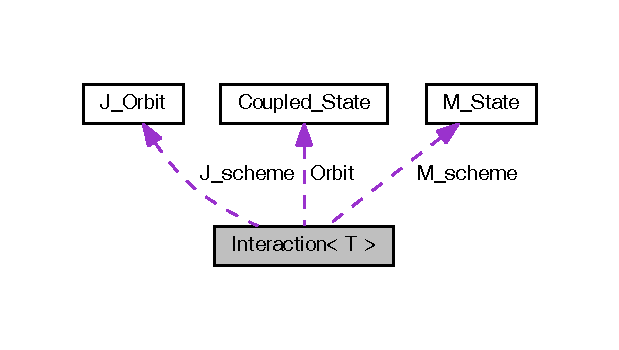
\includegraphics[width=297pt]{class_interaction__coll__graph}
\end{center}
\end{figure}
\subsection*{Public Member Functions}
\begin{DoxyCompactItemize}
\item 
\hyperlink{class_interaction_a1590aded9946d5afaa3ae5a2f77b1933}{Interaction} ()
\item 
\hyperlink{class_interaction_a3579f62f4d43a48f62dab8b5ca560941}{Interaction} (string space, string M\-E, int A)
\item 
\hyperlink{class_interaction_a3d1a04c8afff080d7e9409d59a96efba}{$\sim$\-Interaction} ()
\item 
void \hyperlink{class_interaction_a906559736b06d72e49244436e8dfad0d}{unpack} (int num, int \&i, int \&j, int \&k, int \&l)
\item 
void \hyperlink{class_interaction_a68bde2a8a674f54a8f42cd992e96b907}{pack} (int i, int j, int k, int l, int \&num)
\item 
void \hyperlink{class_interaction_a5215914c0464c733a6c140a814b48513}{Read\-\_\-\-Orbit\-\_\-\-Iso} (string space)
\begin{DoxyCompactList}\small\item\em Read J orbit in isospin representation. \end{DoxyCompactList}\item 
void \hyperlink{class_interaction_a6df2e9326e87a957cf6efd63e3188cf7}{Read\-\_\-\-Orbit\-\_\-\-P\-N} (string space)
\begin{DoxyCompactList}\small\item\em Read J orbit in proton-\/neutron representation. \end{DoxyCompactList}\item 
void \hyperlink{class_interaction_a467419c63d4d647ad219f7b46b6afed5}{Read\-\_\-\-Interaction\-\_\-\-Iso} (string M\-E)
\begin{DoxyCompactList}\small\item\em Read O\-B\-M\-E and T\-B\-M\-E in isospin representation. \end{DoxyCompactList}\item 
void \hyperlink{class_interaction_a96b36b6eab380437ba94585a5ac2a31b}{Read\-\_\-\-Interaction\-\_\-\-P\-N} (string M\-E)
\begin{DoxyCompactList}\small\item\em Read O\-B\-M\-E and T\-B\-M\-E in proton-\/neutron representation. \end{DoxyCompactList}\item 
void \hyperlink{class_interaction_ae6f2362eebdf933d63c8133328fbf0f7}{Construct\-\_\-\-Interaction\-\_\-\-Iso} ()
\begin{DoxyCompactList}\small\item\em Construct interaction in isospin representation. \end{DoxyCompactList}\item 
void \hyperlink{class_interaction_a42aceecb46825fe9c78b71a00f888206}{Construct\-\_\-\-Interaction\-\_\-\-P\-N} ()
\begin{DoxyCompactList}\small\item\em Construct interaction in proton-\/neutron representation. \end{DoxyCompactList}\item 
void \hyperlink{class_interaction_ae16c26ed612f825cfa114b0ca9a4fbc2}{Setup\-\_\-\-Uncoupled\-\_\-\-States\-\_\-\-Iso} (\hyperlink{class_j___orbit}{J\-\_\-\-Orbit} $\ast$J, int dim, \hyperlink{struct_coupled___state}{Coupled\-\_\-\-State} $\ast$vtbme)
\begin{DoxyCompactList}\small\item\em Setup T\-B\-M\-E and uncoupled states in isospin representation. \end{DoxyCompactList}\item 
void \hyperlink{class_interaction_a34f5f4258d6b5acb0cb228ff82855ed6}{Setup\-\_\-\-Uncoupled\-\_\-\-States\-\_\-\-P\-N} (\hyperlink{class_j___orbit}{J\-\_\-\-Orbit} $\ast$$\ast$Jstates, int $\ast$dim, \hyperlink{struct_coupled___state}{Coupled\-\_\-\-State} $\ast$vtbme)
\begin{DoxyCompactList}\small\item\em Setup T\-B\-M\-E and uncoupled states in proton-\/neutron representation. \end{DoxyCompactList}\item 
{\footnotesize template$<$typename T1 , typename T2 , typename T3 $>$ }\\void \hyperlink{class_interaction_aa840d7de0932cb51370619a8033b7800}{Basis\-\_\-\-Transform} (\hyperlink{class_interaction}{Interaction}$<$ T3 $>$ \&force, T1 $\ast$psil, T2 $\ast$psir)
\end{DoxyCompactItemize}
\subsection*{Public Attributes}
\begin{DoxyCompactItemize}
\item 
int \hyperlink{class_interaction_afef136dd95339bef3a8c5e8488f6455f}{Dimension\-\_\-\-M} \mbox{[}\hyperlink{class_interaction_a067c62aec0e8fba647d5e5cefb13fadc}{Iso\-Spin\-\_\-\-Z}\mbox{]}
\item 
int \hyperlink{class_interaction_ae169b32f8b692bdf54bdae97c2f395be}{Dimension\-\_\-\-J} \mbox{[}\hyperlink{class_interaction_a067c62aec0e8fba647d5e5cefb13fadc}{Iso\-Spin\-\_\-\-Z}\mbox{]}
\item 
\hyperlink{class_j___orbit}{J\-\_\-\-Orbit} $\ast$ \hyperlink{class_interaction_a42d5c1378bd17f7755424f7ab5702ef6}{J\-\_\-scheme} \mbox{[}\hyperlink{class_interaction_a067c62aec0e8fba647d5e5cefb13fadc}{Iso\-Spin\-\_\-\-Z}\mbox{]}
\item 
\hyperlink{class_m___state}{M\-\_\-\-State} $\ast$ \hyperlink{class_interaction_ad29cbf9eca392e71958932cef5f7bf66}{M\-\_\-scheme} \mbox{[}\hyperlink{class_interaction_a067c62aec0e8fba647d5e5cefb13fadc}{Iso\-Spin\-\_\-\-Z}\mbox{]}
\item 
ivec \hyperlink{class_interaction_acfc6941cb6a85c4368855da6503a892f}{index} \mbox{[}\hyperlink{class_interaction_a067c62aec0e8fba647d5e5cefb13fadc}{Iso\-Spin\-\_\-\-Z}+1\mbox{]}
\item 
Col$<$ T $>$ \hyperlink{class_interaction_ac7b745819fe9b13f3df3bd7750eceb97}{T\-B\-M\-E} \mbox{[}\hyperlink{class_interaction_a067c62aec0e8fba647d5e5cefb13fadc}{Iso\-Spin\-\_\-\-Z}+1\mbox{]}
\item 
Mat$<$ T $>$ \hyperlink{class_interaction_ad629df71841bfb02116616b2f4764811}{O\-B\-M\-E} \mbox{[}\hyperlink{class_interaction_a067c62aec0e8fba647d5e5cefb13fadc}{Iso\-Spin\-\_\-\-Z}\mbox{]}
\end{DoxyCompactItemize}
\subsection*{Static Public Attributes}
\begin{DoxyCompactItemize}
\item 
static const int \hyperlink{class_interaction_a067c62aec0e8fba647d5e5cefb13fadc}{Iso\-Spin\-\_\-\-Z} = 2
\end{DoxyCompactItemize}
\subsection*{Private Attributes}
\begin{DoxyCompactItemize}
\item 
\hyperlink{struct_coupled___state}{Coupled\-\_\-\-State} $\ast$ \hyperlink{class_interaction_aafd4ee901de0d1463b71f89294b4b3f5}{Orbit}
\item 
int \hyperlink{class_interaction_a5a8eceab2bed942ec46d581b4cd4a661}{Mass\-\_\-\-Num}
\item 
double \hyperlink{class_interaction_afd1f26a552c012f6444e02a0f2718388}{hbar\-\_\-omiga}
\end{DoxyCompactItemize}


\subsection{Constructor \& Destructor Documentation}
\hypertarget{class_interaction_a1590aded9946d5afaa3ae5a2f77b1933}{\index{Interaction@{Interaction}!Interaction@{Interaction}}
\index{Interaction@{Interaction}!Interaction@{Interaction}}
\subsubsection[{Interaction}]{\setlength{\rightskip}{0pt plus 5cm}template$<$typename T $>$ {\bf Interaction}$<$ T $>$\-::{\bf Interaction} (
\begin{DoxyParamCaption}
{}
\end{DoxyParamCaption}
)}}\label{class_interaction_a1590aded9946d5afaa3ae5a2f77b1933}
\hypertarget{class_interaction_a3579f62f4d43a48f62dab8b5ca560941}{\index{Interaction@{Interaction}!Interaction@{Interaction}}
\index{Interaction@{Interaction}!Interaction@{Interaction}}
\subsubsection[{Interaction}]{\setlength{\rightskip}{0pt plus 5cm}template$<$typename T $>$ {\bf Interaction}$<$ T $>$\-::{\bf Interaction} (
\begin{DoxyParamCaption}
\item[{string}]{space, }
\item[{string}]{M\-E, }
\item[{int}]{A}
\end{DoxyParamCaption}
)}}\label{class_interaction_a3579f62f4d43a48f62dab8b5ca560941}


Here is the call graph for this function\-:
\nopagebreak
\begin{figure}[H]
\begin{center}
\leavevmode
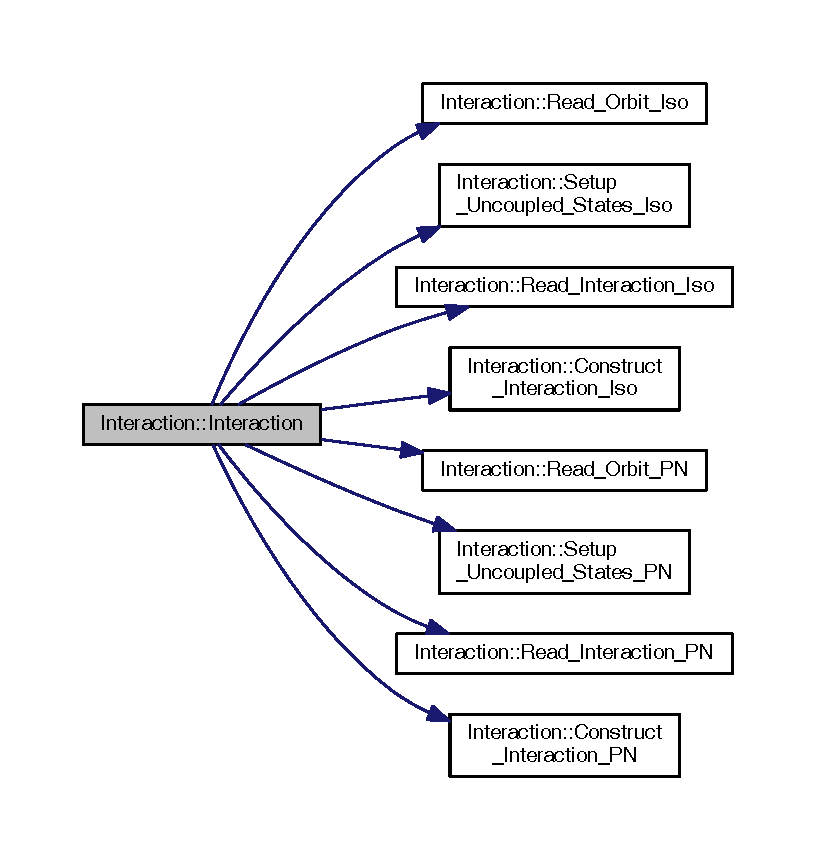
\includegraphics[width=350pt]{class_interaction_a3579f62f4d43a48f62dab8b5ca560941_cgraph}
\end{center}
\end{figure}


\hypertarget{class_interaction_a3d1a04c8afff080d7e9409d59a96efba}{\index{Interaction@{Interaction}!$\sim$\-Interaction@{$\sim$\-Interaction}}
\index{$\sim$\-Interaction@{$\sim$\-Interaction}!Interaction@{Interaction}}
\subsubsection[{$\sim$\-Interaction}]{\setlength{\rightskip}{0pt plus 5cm}template$<$typename T $>$ {\bf Interaction}$<$ T $>$\-::$\sim${\bf Interaction} (
\begin{DoxyParamCaption}
{}
\end{DoxyParamCaption}
)}}\label{class_interaction_a3d1a04c8afff080d7e9409d59a96efba}


\subsection{Member Function Documentation}
\hypertarget{class_interaction_aa840d7de0932cb51370619a8033b7800}{\index{Interaction@{Interaction}!Basis\-\_\-\-Transform@{Basis\-\_\-\-Transform}}
\index{Basis\-\_\-\-Transform@{Basis\-\_\-\-Transform}!Interaction@{Interaction}}
\subsubsection[{Basis\-\_\-\-Transform}]{\setlength{\rightskip}{0pt plus 5cm}template$<$typename T $>$ template$<$typename T1 , typename T2 , typename T3 $>$ void {\bf Interaction}$<$ T $>$\-::Basis\-\_\-\-Transform (
\begin{DoxyParamCaption}
\item[{{\bf Interaction}$<$ T3 $>$ \&}]{force, }
\item[{T1 $\ast$}]{psil, }
\item[{T2 $\ast$}]{psir}
\end{DoxyParamCaption}
)}}\label{class_interaction_aa840d7de0932cb51370619a8033b7800}
One body matrix elements

Two body matrix elements 

Here is the call graph for this function\-:
\nopagebreak
\begin{figure}[H]
\begin{center}
\leavevmode
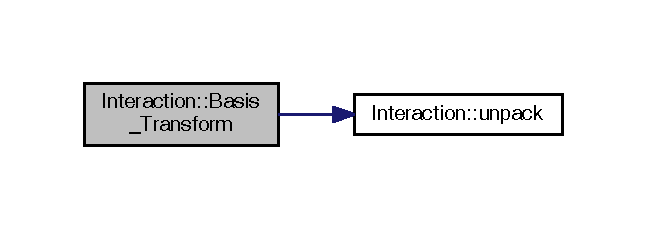
\includegraphics[width=310pt]{class_interaction_aa840d7de0932cb51370619a8033b7800_cgraph}
\end{center}
\end{figure}




Here is the caller graph for this function\-:
\nopagebreak
\begin{figure}[H]
\begin{center}
\leavevmode
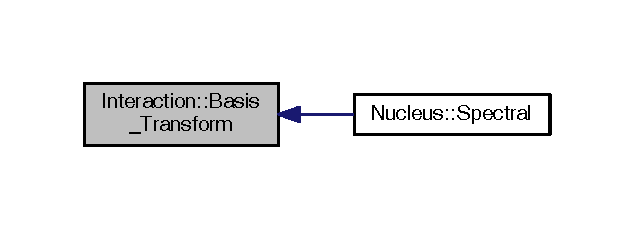
\includegraphics[width=304pt]{class_interaction_aa840d7de0932cb51370619a8033b7800_icgraph}
\end{center}
\end{figure}


\hypertarget{class_interaction_ae6f2362eebdf933d63c8133328fbf0f7}{\index{Interaction@{Interaction}!Construct\-\_\-\-Interaction\-\_\-\-Iso@{Construct\-\_\-\-Interaction\-\_\-\-Iso}}
\index{Construct\-\_\-\-Interaction\-\_\-\-Iso@{Construct\-\_\-\-Interaction\-\_\-\-Iso}!Interaction@{Interaction}}
\subsubsection[{Construct\-\_\-\-Interaction\-\_\-\-Iso}]{\setlength{\rightskip}{0pt plus 5cm}template$<$typename T $>$ void {\bf Interaction}$<$ T $>$\-::Construct\-\_\-\-Interaction\-\_\-\-Iso (
\begin{DoxyParamCaption}
{}
\end{DoxyParamCaption}
)}}\label{class_interaction_ae6f2362eebdf933d63c8133328fbf0f7}


Construct interaction in isospin representation. 


\begin{DoxyParams}{Parameters}
{\em T\-B\-M\-E} & J scheme \\
\hline
\end{DoxyParams}
\begin{DoxyReturn}{Returns}
T\-B\-M\-E M scheme 
\end{DoxyReturn}
pp, nn interaction

pn interaction 

Here is the caller graph for this function\-:
\nopagebreak
\begin{figure}[H]
\begin{center}
\leavevmode
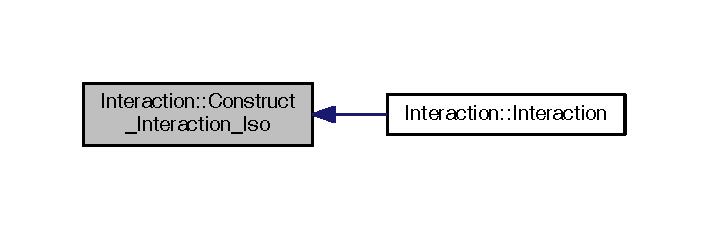
\includegraphics[width=340pt]{class_interaction_ae6f2362eebdf933d63c8133328fbf0f7_icgraph}
\end{center}
\end{figure}


\hypertarget{class_interaction_a42aceecb46825fe9c78b71a00f888206}{\index{Interaction@{Interaction}!Construct\-\_\-\-Interaction\-\_\-\-P\-N@{Construct\-\_\-\-Interaction\-\_\-\-P\-N}}
\index{Construct\-\_\-\-Interaction\-\_\-\-P\-N@{Construct\-\_\-\-Interaction\-\_\-\-P\-N}!Interaction@{Interaction}}
\subsubsection[{Construct\-\_\-\-Interaction\-\_\-\-P\-N}]{\setlength{\rightskip}{0pt plus 5cm}template$<$typename T $>$ void {\bf Interaction}$<$ T $>$\-::Construct\-\_\-\-Interaction\-\_\-\-P\-N (
\begin{DoxyParamCaption}
{}
\end{DoxyParamCaption}
)}}\label{class_interaction_a42aceecb46825fe9c78b71a00f888206}


Construct interaction in proton-\/neutron representation. 


\begin{DoxyParams}{Parameters}
{\em T\-B\-M\-E} & J scheme \\
\hline
\end{DoxyParams}
\begin{DoxyReturn}{Returns}
T\-B\-M\-E M scheme 
\end{DoxyReturn}
pp, nn interaction

pn interaction

if(oa==ob) fact$\ast$=sqrt(2.\-0); if(oc==od) fact$\ast$=sqrt(2.\-0);

!!!5 

Here is the caller graph for this function\-:
\nopagebreak
\begin{figure}[H]
\begin{center}
\leavevmode
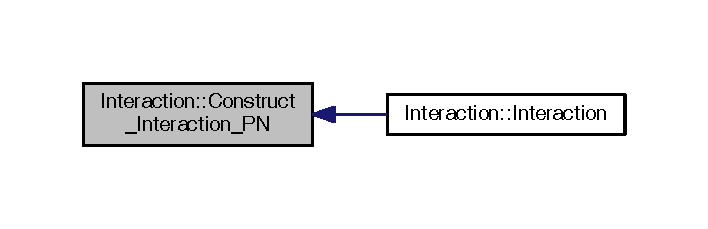
\includegraphics[width=340pt]{class_interaction_a42aceecb46825fe9c78b71a00f888206_icgraph}
\end{center}
\end{figure}


\hypertarget{class_interaction_a68bde2a8a674f54a8f42cd992e96b907}{\index{Interaction@{Interaction}!pack@{pack}}
\index{pack@{pack}!Interaction@{Interaction}}
\subsubsection[{pack}]{\setlength{\rightskip}{0pt plus 5cm}template$<$typename T $>$ void {\bf Interaction}$<$ T $>$\-::pack (
\begin{DoxyParamCaption}
\item[{int}]{i, }
\item[{int}]{j, }
\item[{int}]{k, }
\item[{int}]{l, }
\item[{int \&}]{num}
\end{DoxyParamCaption}
)}}\label{class_interaction_a68bde2a8a674f54a8f42cd992e96b907}
\hypertarget{class_interaction_a467419c63d4d647ad219f7b46b6afed5}{\index{Interaction@{Interaction}!Read\-\_\-\-Interaction\-\_\-\-Iso@{Read\-\_\-\-Interaction\-\_\-\-Iso}}
\index{Read\-\_\-\-Interaction\-\_\-\-Iso@{Read\-\_\-\-Interaction\-\_\-\-Iso}!Interaction@{Interaction}}
\subsubsection[{Read\-\_\-\-Interaction\-\_\-\-Iso}]{\setlength{\rightskip}{0pt plus 5cm}template$<$typename T $>$ void {\bf Interaction}$<$ T $>$\-::Read\-\_\-\-Interaction\-\_\-\-Iso (
\begin{DoxyParamCaption}
\item[{string}]{M\-E}
\end{DoxyParamCaption}
)}}\label{class_interaction_a467419c63d4d647ad219f7b46b6afed5}


Read O\-B\-M\-E and T\-B\-M\-E in isospin representation. 


\begin{DoxyParams}{Parameters}
{\em Martrix\-Elements} & \\
\hline
\end{DoxyParams}
\begin{DoxyReturn}{Returns}
O\-B\-M\-E 

T\-B\-M\-E J scheme 
\end{DoxyReturn}


Here is the caller graph for this function\-:
\nopagebreak
\begin{figure}[H]
\begin{center}
\leavevmode
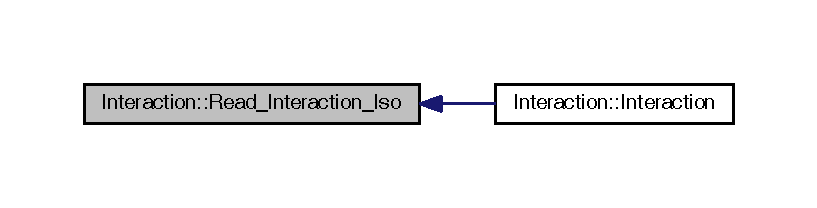
\includegraphics[width=350pt]{class_interaction_a467419c63d4d647ad219f7b46b6afed5_icgraph}
\end{center}
\end{figure}


\hypertarget{class_interaction_a96b36b6eab380437ba94585a5ac2a31b}{\index{Interaction@{Interaction}!Read\-\_\-\-Interaction\-\_\-\-P\-N@{Read\-\_\-\-Interaction\-\_\-\-P\-N}}
\index{Read\-\_\-\-Interaction\-\_\-\-P\-N@{Read\-\_\-\-Interaction\-\_\-\-P\-N}!Interaction@{Interaction}}
\subsubsection[{Read\-\_\-\-Interaction\-\_\-\-P\-N}]{\setlength{\rightskip}{0pt plus 5cm}template$<$typename T $>$ void {\bf Interaction}$<$ T $>$\-::Read\-\_\-\-Interaction\-\_\-\-P\-N (
\begin{DoxyParamCaption}
\item[{string}]{M\-E}
\end{DoxyParamCaption}
)}}\label{class_interaction_a96b36b6eab380437ba94585a5ac2a31b}


Read O\-B\-M\-E and T\-B\-M\-E in proton-\/neutron representation. 


\begin{DoxyParams}{Parameters}
{\em Martrix\-Elements} & \\
\hline
\end{DoxyParams}
\begin{DoxyReturn}{Returns}
O\-B\-M\-E 

T\-B\-M\-E J scheme 
\end{DoxyReturn}


Here is the caller graph for this function\-:
\nopagebreak
\begin{figure}[H]
\begin{center}
\leavevmode
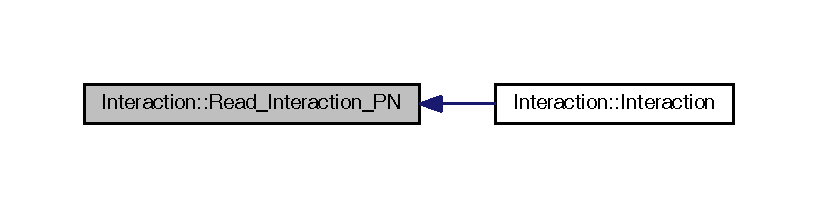
\includegraphics[width=350pt]{class_interaction_a96b36b6eab380437ba94585a5ac2a31b_icgraph}
\end{center}
\end{figure}


\hypertarget{class_interaction_a5215914c0464c733a6c140a814b48513}{\index{Interaction@{Interaction}!Read\-\_\-\-Orbit\-\_\-\-Iso@{Read\-\_\-\-Orbit\-\_\-\-Iso}}
\index{Read\-\_\-\-Orbit\-\_\-\-Iso@{Read\-\_\-\-Orbit\-\_\-\-Iso}!Interaction@{Interaction}}
\subsubsection[{Read\-\_\-\-Orbit\-\_\-\-Iso}]{\setlength{\rightskip}{0pt plus 5cm}template$<$typename T $>$ void {\bf Interaction}$<$ T $>$\-::Read\-\_\-\-Orbit\-\_\-\-Iso (
\begin{DoxyParamCaption}
\item[{string}]{space}
\end{DoxyParamCaption}
)}}\label{class_interaction_a5215914c0464c733a6c140a814b48513}


Read J orbit in isospin representation. 

\begin{DoxyReturn}{Returns}
\hyperlink{class_j___orbit}{J\-\_\-\-Orbit} 
\end{DoxyReturn}


Here is the caller graph for this function\-:
\nopagebreak
\begin{figure}[H]
\begin{center}
\leavevmode
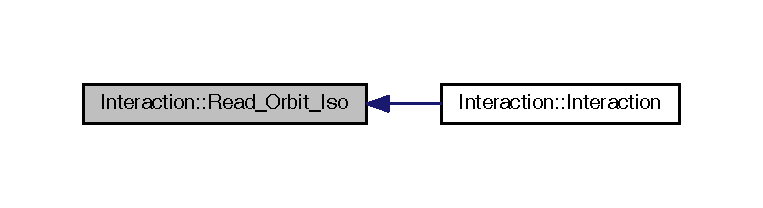
\includegraphics[width=350pt]{class_interaction_a5215914c0464c733a6c140a814b48513_icgraph}
\end{center}
\end{figure}


\hypertarget{class_interaction_a6df2e9326e87a957cf6efd63e3188cf7}{\index{Interaction@{Interaction}!Read\-\_\-\-Orbit\-\_\-\-P\-N@{Read\-\_\-\-Orbit\-\_\-\-P\-N}}
\index{Read\-\_\-\-Orbit\-\_\-\-P\-N@{Read\-\_\-\-Orbit\-\_\-\-P\-N}!Interaction@{Interaction}}
\subsubsection[{Read\-\_\-\-Orbit\-\_\-\-P\-N}]{\setlength{\rightskip}{0pt plus 5cm}template$<$typename T $>$ void {\bf Interaction}$<$ T $>$\-::Read\-\_\-\-Orbit\-\_\-\-P\-N (
\begin{DoxyParamCaption}
\item[{string}]{space}
\end{DoxyParamCaption}
)}}\label{class_interaction_a6df2e9326e87a957cf6efd63e3188cf7}


Read J orbit in proton-\/neutron representation. 

\begin{DoxyReturn}{Returns}
\hyperlink{class_j___orbit}{J\-\_\-\-Orbit} 
\end{DoxyReturn}


Here is the caller graph for this function\-:
\nopagebreak
\begin{figure}[H]
\begin{center}
\leavevmode
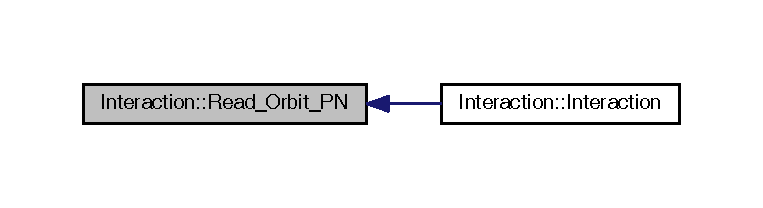
\includegraphics[width=350pt]{class_interaction_a6df2e9326e87a957cf6efd63e3188cf7_icgraph}
\end{center}
\end{figure}


\hypertarget{class_interaction_ae16c26ed612f825cfa114b0ca9a4fbc2}{\index{Interaction@{Interaction}!Setup\-\_\-\-Uncoupled\-\_\-\-States\-\_\-\-Iso@{Setup\-\_\-\-Uncoupled\-\_\-\-States\-\_\-\-Iso}}
\index{Setup\-\_\-\-Uncoupled\-\_\-\-States\-\_\-\-Iso@{Setup\-\_\-\-Uncoupled\-\_\-\-States\-\_\-\-Iso}!Interaction@{Interaction}}
\subsubsection[{Setup\-\_\-\-Uncoupled\-\_\-\-States\-\_\-\-Iso}]{\setlength{\rightskip}{0pt plus 5cm}template$<$typename T $>$ void {\bf Interaction}$<$ T $>$\-::Setup\-\_\-\-Uncoupled\-\_\-\-States\-\_\-\-Iso (
\begin{DoxyParamCaption}
\item[{{\bf J\-\_\-\-Orbit} $\ast$}]{Jstates, }
\item[{int}]{dim, }
\item[{{\bf Coupled\-\_\-\-State} $\ast$}]{vtbme}
\end{DoxyParamCaption}
)}}\label{class_interaction_ae16c26ed612f825cfa114b0ca9a4fbc2}


Setup T\-B\-M\-E and uncoupled states in isospin representation. 


\begin{DoxyParams}{Parameters}
{\em \hyperlink{class_j___orbit}{J\-\_\-\-Orbit}} & \\
\hline
\end{DoxyParams}
\begin{DoxyReturn}{Returns}
T\-B\-M\-E space 
\end{DoxyReturn}


Here is the caller graph for this function\-:
\nopagebreak
\begin{figure}[H]
\begin{center}
\leavevmode
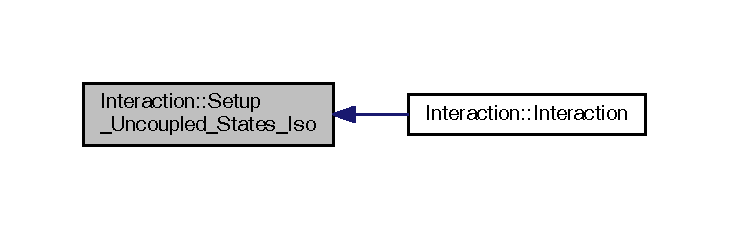
\includegraphics[width=350pt]{class_interaction_ae16c26ed612f825cfa114b0ca9a4fbc2_icgraph}
\end{center}
\end{figure}


\hypertarget{class_interaction_a34f5f4258d6b5acb0cb228ff82855ed6}{\index{Interaction@{Interaction}!Setup\-\_\-\-Uncoupled\-\_\-\-States\-\_\-\-P\-N@{Setup\-\_\-\-Uncoupled\-\_\-\-States\-\_\-\-P\-N}}
\index{Setup\-\_\-\-Uncoupled\-\_\-\-States\-\_\-\-P\-N@{Setup\-\_\-\-Uncoupled\-\_\-\-States\-\_\-\-P\-N}!Interaction@{Interaction}}
\subsubsection[{Setup\-\_\-\-Uncoupled\-\_\-\-States\-\_\-\-P\-N}]{\setlength{\rightskip}{0pt plus 5cm}template$<$typename T $>$ void {\bf Interaction}$<$ T $>$\-::Setup\-\_\-\-Uncoupled\-\_\-\-States\-\_\-\-P\-N (
\begin{DoxyParamCaption}
\item[{{\bf J\-\_\-\-Orbit} $\ast$$\ast$}]{Jstates, }
\item[{int $\ast$}]{dim, }
\item[{{\bf Coupled\-\_\-\-State} $\ast$}]{vtbme}
\end{DoxyParamCaption}
)}}\label{class_interaction_a34f5f4258d6b5acb0cb228ff82855ed6}


Setup T\-B\-M\-E and uncoupled states in proton-\/neutron representation. 


\begin{DoxyParams}{Parameters}
{\em \hyperlink{class_j___orbit}{J\-\_\-\-Orbit}} & \\
\hline
\end{DoxyParams}
\begin{DoxyReturn}{Returns}
T\-B\-M\-E space 
\end{DoxyReturn}


Here is the caller graph for this function\-:
\nopagebreak
\begin{figure}[H]
\begin{center}
\leavevmode
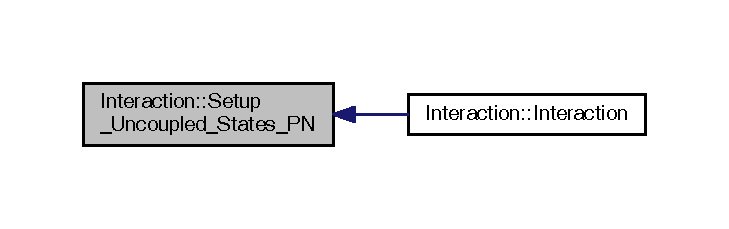
\includegraphics[width=350pt]{class_interaction_a34f5f4258d6b5acb0cb228ff82855ed6_icgraph}
\end{center}
\end{figure}


\hypertarget{class_interaction_a906559736b06d72e49244436e8dfad0d}{\index{Interaction@{Interaction}!unpack@{unpack}}
\index{unpack@{unpack}!Interaction@{Interaction}}
\subsubsection[{unpack}]{\setlength{\rightskip}{0pt plus 5cm}template$<$typename T $>$ void {\bf Interaction}$<$ T $>$\-::unpack (
\begin{DoxyParamCaption}
\item[{int}]{num, }
\item[{int \&}]{i, }
\item[{int \&}]{j, }
\item[{int \&}]{k, }
\item[{int \&}]{l}
\end{DoxyParamCaption}
)}}\label{class_interaction_a906559736b06d72e49244436e8dfad0d}


Here is the caller graph for this function\-:
\nopagebreak
\begin{figure}[H]
\begin{center}
\leavevmode
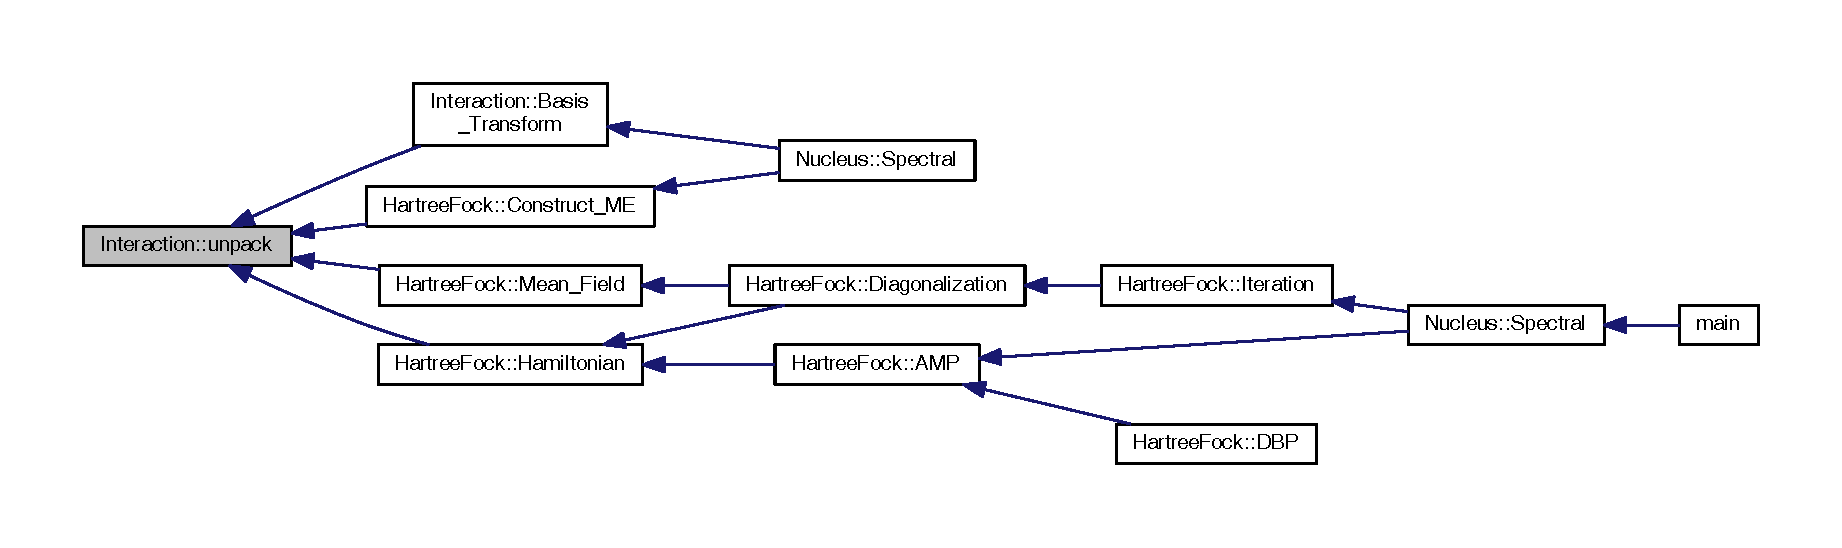
\includegraphics[width=350pt]{class_interaction_a906559736b06d72e49244436e8dfad0d_icgraph}
\end{center}
\end{figure}




\subsection{Member Data Documentation}
\hypertarget{class_interaction_ae169b32f8b692bdf54bdae97c2f395be}{\index{Interaction@{Interaction}!Dimension\-\_\-\-J@{Dimension\-\_\-\-J}}
\index{Dimension\-\_\-\-J@{Dimension\-\_\-\-J}!Interaction@{Interaction}}
\subsubsection[{Dimension\-\_\-\-J}]{\setlength{\rightskip}{0pt plus 5cm}template$<$typename T$>$ int {\bf Interaction}$<$ T $>$\-::Dimension\-\_\-\-J\mbox{[}{\bf Iso\-Spin\-\_\-\-Z}\mbox{]}}}\label{class_interaction_ae169b32f8b692bdf54bdae97c2f395be}
\hypertarget{class_interaction_afef136dd95339bef3a8c5e8488f6455f}{\index{Interaction@{Interaction}!Dimension\-\_\-\-M@{Dimension\-\_\-\-M}}
\index{Dimension\-\_\-\-M@{Dimension\-\_\-\-M}!Interaction@{Interaction}}
\subsubsection[{Dimension\-\_\-\-M}]{\setlength{\rightskip}{0pt plus 5cm}template$<$typename T$>$ int {\bf Interaction}$<$ T $>$\-::Dimension\-\_\-\-M\mbox{[}{\bf Iso\-Spin\-\_\-\-Z}\mbox{]}}}\label{class_interaction_afef136dd95339bef3a8c5e8488f6455f}
\hypertarget{class_interaction_afd1f26a552c012f6444e02a0f2718388}{\index{Interaction@{Interaction}!hbar\-\_\-omiga@{hbar\-\_\-omiga}}
\index{hbar\-\_\-omiga@{hbar\-\_\-omiga}!Interaction@{Interaction}}
\subsubsection[{hbar\-\_\-omiga}]{\setlength{\rightskip}{0pt plus 5cm}template$<$typename T$>$ double {\bf Interaction}$<$ T $>$\-::hbar\-\_\-omiga\hspace{0.3cm}{\ttfamily [private]}}}\label{class_interaction_afd1f26a552c012f6444e02a0f2718388}
\hypertarget{class_interaction_acfc6941cb6a85c4368855da6503a892f}{\index{Interaction@{Interaction}!index@{index}}
\index{index@{index}!Interaction@{Interaction}}
\subsubsection[{index}]{\setlength{\rightskip}{0pt plus 5cm}template$<$typename T$>$ ivec {\bf Interaction}$<$ T $>$\-::index\mbox{[}{\bf Iso\-Spin\-\_\-\-Z}+1\mbox{]}}}\label{class_interaction_acfc6941cb6a85c4368855da6503a892f}
\hypertarget{class_interaction_a067c62aec0e8fba647d5e5cefb13fadc}{\index{Interaction@{Interaction}!Iso\-Spin\-\_\-\-Z@{Iso\-Spin\-\_\-\-Z}}
\index{Iso\-Spin\-\_\-\-Z@{Iso\-Spin\-\_\-\-Z}!Interaction@{Interaction}}
\subsubsection[{Iso\-Spin\-\_\-\-Z}]{\setlength{\rightskip}{0pt plus 5cm}template$<$typename T$>$ const int {\bf Interaction}$<$ T $>$\-::Iso\-Spin\-\_\-\-Z = 2\hspace{0.3cm}{\ttfamily [static]}}}\label{class_interaction_a067c62aec0e8fba647d5e5cefb13fadc}
\hypertarget{class_interaction_a42d5c1378bd17f7755424f7ab5702ef6}{\index{Interaction@{Interaction}!J\-\_\-scheme@{J\-\_\-scheme}}
\index{J\-\_\-scheme@{J\-\_\-scheme}!Interaction@{Interaction}}
\subsubsection[{J\-\_\-scheme}]{\setlength{\rightskip}{0pt plus 5cm}template$<$typename T$>$ {\bf J\-\_\-\-Orbit}$\ast$ {\bf Interaction}$<$ T $>$\-::J\-\_\-scheme\mbox{[}{\bf Iso\-Spin\-\_\-\-Z}\mbox{]}}}\label{class_interaction_a42d5c1378bd17f7755424f7ab5702ef6}
\hypertarget{class_interaction_ad29cbf9eca392e71958932cef5f7bf66}{\index{Interaction@{Interaction}!M\-\_\-scheme@{M\-\_\-scheme}}
\index{M\-\_\-scheme@{M\-\_\-scheme}!Interaction@{Interaction}}
\subsubsection[{M\-\_\-scheme}]{\setlength{\rightskip}{0pt plus 5cm}template$<$typename T$>$ {\bf M\-\_\-\-State}$\ast$ {\bf Interaction}$<$ T $>$\-::M\-\_\-scheme\mbox{[}{\bf Iso\-Spin\-\_\-\-Z}\mbox{]}}}\label{class_interaction_ad29cbf9eca392e71958932cef5f7bf66}
\hypertarget{class_interaction_a5a8eceab2bed942ec46d581b4cd4a661}{\index{Interaction@{Interaction}!Mass\-\_\-\-Num@{Mass\-\_\-\-Num}}
\index{Mass\-\_\-\-Num@{Mass\-\_\-\-Num}!Interaction@{Interaction}}
\subsubsection[{Mass\-\_\-\-Num}]{\setlength{\rightskip}{0pt plus 5cm}template$<$typename T$>$ int {\bf Interaction}$<$ T $>$\-::Mass\-\_\-\-Num\hspace{0.3cm}{\ttfamily [private]}}}\label{class_interaction_a5a8eceab2bed942ec46d581b4cd4a661}
\hypertarget{class_interaction_ad629df71841bfb02116616b2f4764811}{\index{Interaction@{Interaction}!O\-B\-M\-E@{O\-B\-M\-E}}
\index{O\-B\-M\-E@{O\-B\-M\-E}!Interaction@{Interaction}}
\subsubsection[{O\-B\-M\-E}]{\setlength{\rightskip}{0pt plus 5cm}template$<$typename T$>$ Mat$<$T$>$ {\bf Interaction}$<$ T $>$\-::O\-B\-M\-E\mbox{[}{\bf Iso\-Spin\-\_\-\-Z}\mbox{]}}}\label{class_interaction_ad629df71841bfb02116616b2f4764811}
\hypertarget{class_interaction_aafd4ee901de0d1463b71f89294b4b3f5}{\index{Interaction@{Interaction}!Orbit@{Orbit}}
\index{Orbit@{Orbit}!Interaction@{Interaction}}
\subsubsection[{Orbit}]{\setlength{\rightskip}{0pt plus 5cm}template$<$typename T$>$ {\bf Coupled\-\_\-\-State}$\ast$ {\bf Interaction}$<$ T $>$\-::Orbit\hspace{0.3cm}{\ttfamily [private]}}}\label{class_interaction_aafd4ee901de0d1463b71f89294b4b3f5}
\hypertarget{class_interaction_ac7b745819fe9b13f3df3bd7750eceb97}{\index{Interaction@{Interaction}!T\-B\-M\-E@{T\-B\-M\-E}}
\index{T\-B\-M\-E@{T\-B\-M\-E}!Interaction@{Interaction}}
\subsubsection[{T\-B\-M\-E}]{\setlength{\rightskip}{0pt plus 5cm}template$<$typename T$>$ Col$<$T$>$ {\bf Interaction}$<$ T $>$\-::T\-B\-M\-E\mbox{[}{\bf Iso\-Spin\-\_\-\-Z}+1\mbox{]}}}\label{class_interaction_ac7b745819fe9b13f3df3bd7750eceb97}


The documentation for this class was generated from the following file\-:\begin{DoxyCompactItemize}
\item 
\hyperlink{main_8cpp}{main.\-cpp}\end{DoxyCompactItemize}

\hypertarget{class_j___orbit}{\section{J\-\_\-\-Orbit Class Reference}
\label{class_j___orbit}\index{J\-\_\-\-Orbit@{J\-\_\-\-Orbit}}
}
\subsection*{Public Member Functions}
\begin{DoxyCompactItemize}
\item 
void \hyperlink{class_j___orbit_a48daa459ba3f355a29cae35c22c69354}{set} (int node, int orbit, double angular)
\end{DoxyCompactItemize}
\subsection*{Public Attributes}
\begin{DoxyCompactItemize}
\item 
int \hyperlink{class_j___orbit_abbbbfd967a5f2d1de6e8a1dbd458ee65}{n}
\item 
int \hyperlink{class_j___orbit_a975b5fff0c2c2f6366ff4b1cb6f867f3}{l}
\item 
double \hyperlink{class_j___orbit_a4df41865c99b0ffd1560a388eb67ee44}{j}
\end{DoxyCompactItemize}


\subsection{Member Function Documentation}
\hypertarget{class_j___orbit_a48daa459ba3f355a29cae35c22c69354}{\index{J\-\_\-\-Orbit@{J\-\_\-\-Orbit}!set@{set}}
\index{set@{set}!J_Orbit@{J\-\_\-\-Orbit}}
\subsubsection[{set}]{\setlength{\rightskip}{0pt plus 5cm}void J\-\_\-\-Orbit\-::set (
\begin{DoxyParamCaption}
\item[{int}]{node, }
\item[{int}]{orbit, }
\item[{double}]{angular}
\end{DoxyParamCaption}
)}}\label{class_j___orbit_a48daa459ba3f355a29cae35c22c69354}


\subsection{Member Data Documentation}
\hypertarget{class_j___orbit_a4df41865c99b0ffd1560a388eb67ee44}{\index{J\-\_\-\-Orbit@{J\-\_\-\-Orbit}!j@{j}}
\index{j@{j}!J_Orbit@{J\-\_\-\-Orbit}}
\subsubsection[{j}]{\setlength{\rightskip}{0pt plus 5cm}double J\-\_\-\-Orbit\-::j}}\label{class_j___orbit_a4df41865c99b0ffd1560a388eb67ee44}
\hypertarget{class_j___orbit_a975b5fff0c2c2f6366ff4b1cb6f867f3}{\index{J\-\_\-\-Orbit@{J\-\_\-\-Orbit}!l@{l}}
\index{l@{l}!J_Orbit@{J\-\_\-\-Orbit}}
\subsubsection[{l}]{\setlength{\rightskip}{0pt plus 5cm}int J\-\_\-\-Orbit\-::l}}\label{class_j___orbit_a975b5fff0c2c2f6366ff4b1cb6f867f3}
\hypertarget{class_j___orbit_abbbbfd967a5f2d1de6e8a1dbd458ee65}{\index{J\-\_\-\-Orbit@{J\-\_\-\-Orbit}!n@{n}}
\index{n@{n}!J_Orbit@{J\-\_\-\-Orbit}}
\subsubsection[{n}]{\setlength{\rightskip}{0pt plus 5cm}int J\-\_\-\-Orbit\-::n}}\label{class_j___orbit_abbbbfd967a5f2d1de6e8a1dbd458ee65}


The documentation for this class was generated from the following file\-:\begin{DoxyCompactItemize}
\item 
\hyperlink{main_8cpp}{main.\-cpp}\end{DoxyCompactItemize}

\hypertarget{class_m___state}{\section{M\-\_\-\-State Class Reference}
\label{class_m___state}\index{M\-\_\-\-State@{M\-\_\-\-State}}
}
\subsection*{Public Member Functions}
\begin{DoxyCompactItemize}
\item 
void \hyperlink{class_m___state_a11c3f1e264eaae5323063825131320eb}{set} (int i, int node, int orbit, double angular, double jz, double pn)
\end{DoxyCompactItemize}
\subsection*{Public Attributes}
\begin{DoxyCompactItemize}
\item 
int \hyperlink{class_m___state_a7d8b37c43bf4afe490abd8d8b9f8a292}{index}
\item 
int \hyperlink{class_m___state_a27fbcff7783c0ebb82bb04452cdc573b}{n}
\item 
int \hyperlink{class_m___state_ad2ba5c44ffd8c57842b2cbd8ddabda4b}{l}
\item 
double \hyperlink{class_m___state_a2f5230904bf6ba0c74f9d1bed5e8229d}{j}
\item 
double \hyperlink{class_m___state_a2c76c65cf0d884bc8de693c3db782028}{m}
\item 
double \hyperlink{class_m___state_adf6969c1f683828c2968ca892ef039cf}{Iz}
\end{DoxyCompactItemize}


\subsection{Member Function Documentation}
\hypertarget{class_m___state_a11c3f1e264eaae5323063825131320eb}{\index{M\-\_\-\-State@{M\-\_\-\-State}!set@{set}}
\index{set@{set}!M_State@{M\-\_\-\-State}}
\subsubsection[{set}]{\setlength{\rightskip}{0pt plus 5cm}void M\-\_\-\-State\-::set (
\begin{DoxyParamCaption}
\item[{int}]{i, }
\item[{int}]{node, }
\item[{int}]{orbit, }
\item[{double}]{angular, }
\item[{double}]{jz, }
\item[{double}]{pn}
\end{DoxyParamCaption}
)}}\label{class_m___state_a11c3f1e264eaae5323063825131320eb}


\subsection{Member Data Documentation}
\hypertarget{class_m___state_a7d8b37c43bf4afe490abd8d8b9f8a292}{\index{M\-\_\-\-State@{M\-\_\-\-State}!index@{index}}
\index{index@{index}!M_State@{M\-\_\-\-State}}
\subsubsection[{index}]{\setlength{\rightskip}{0pt plus 5cm}int M\-\_\-\-State\-::index}}\label{class_m___state_a7d8b37c43bf4afe490abd8d8b9f8a292}
\hypertarget{class_m___state_adf6969c1f683828c2968ca892ef039cf}{\index{M\-\_\-\-State@{M\-\_\-\-State}!Iz@{Iz}}
\index{Iz@{Iz}!M_State@{M\-\_\-\-State}}
\subsubsection[{Iz}]{\setlength{\rightskip}{0pt plus 5cm}double M\-\_\-\-State\-::\-Iz}}\label{class_m___state_adf6969c1f683828c2968ca892ef039cf}
\hypertarget{class_m___state_a2f5230904bf6ba0c74f9d1bed5e8229d}{\index{M\-\_\-\-State@{M\-\_\-\-State}!j@{j}}
\index{j@{j}!M_State@{M\-\_\-\-State}}
\subsubsection[{j}]{\setlength{\rightskip}{0pt plus 5cm}double M\-\_\-\-State\-::j}}\label{class_m___state_a2f5230904bf6ba0c74f9d1bed5e8229d}
\hypertarget{class_m___state_ad2ba5c44ffd8c57842b2cbd8ddabda4b}{\index{M\-\_\-\-State@{M\-\_\-\-State}!l@{l}}
\index{l@{l}!M_State@{M\-\_\-\-State}}
\subsubsection[{l}]{\setlength{\rightskip}{0pt plus 5cm}int M\-\_\-\-State\-::l}}\label{class_m___state_ad2ba5c44ffd8c57842b2cbd8ddabda4b}
\hypertarget{class_m___state_a2c76c65cf0d884bc8de693c3db782028}{\index{M\-\_\-\-State@{M\-\_\-\-State}!m@{m}}
\index{m@{m}!M_State@{M\-\_\-\-State}}
\subsubsection[{m}]{\setlength{\rightskip}{0pt plus 5cm}double M\-\_\-\-State\-::m}}\label{class_m___state_a2c76c65cf0d884bc8de693c3db782028}
\hypertarget{class_m___state_a27fbcff7783c0ebb82bb04452cdc573b}{\index{M\-\_\-\-State@{M\-\_\-\-State}!n@{n}}
\index{n@{n}!M_State@{M\-\_\-\-State}}
\subsubsection[{n}]{\setlength{\rightskip}{0pt plus 5cm}int M\-\_\-\-State\-::n}}\label{class_m___state_a27fbcff7783c0ebb82bb04452cdc573b}


The documentation for this class was generated from the following file\-:\begin{DoxyCompactItemize}
\item 
\hyperlink{main_8cpp}{main.\-cpp}\end{DoxyCompactItemize}

\hypertarget{class_nucleus}{\section{Nucleus Class Reference}
\label{class_nucleus}\index{Nucleus@{Nucleus}}
}


Collaboration diagram for Nucleus\-:
\nopagebreak
\begin{figure}[H]
\begin{center}
\leavevmode
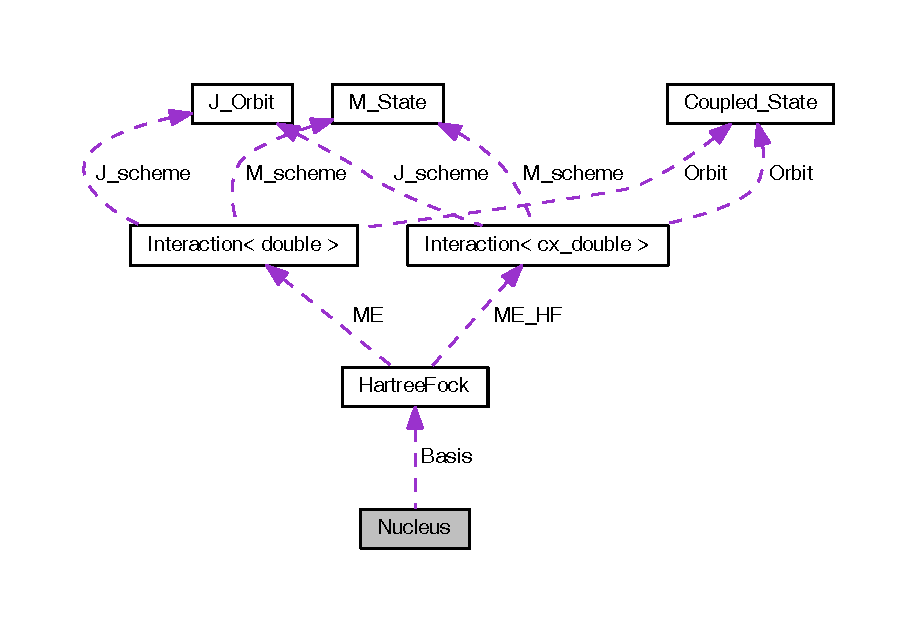
\includegraphics[width=350pt]{class_nucleus__coll__graph}
\end{center}
\end{figure}
\subsection*{Public Member Functions}
\begin{DoxyCompactItemize}
\item 
\hyperlink{class_nucleus_aa51f8aa0e853d8c58c8bbf7e56eb93f9}{Nucleus} (int Z, int A, string space, string force)
\item 
\hyperlink{class_nucleus_a012f1716baa1cf5317e6fc0e06c44647}{$\sim$\-Nucleus} ()
\item 
void \hyperlink{class_nucleus_a5f953c3273fccb833c90c929e6c991a2}{Construct\-\_\-\-Configuration} (vec \&E\-\_\-cutoff)
\begin{DoxyCompactList}\small\item\em Construct different configurations. \end{DoxyCompactList}\item 
void \hyperlink{class_nucleus_a5e449f1e876db72824f9466131becac0}{Spectral} (vec \&J, vec \&Parity)
\begin{DoxyCompactList}\small\item\em Spectral with angular momentum projection. \end{DoxyCompactList}\item 
void \hyperlink{class_nucleus_a2f41a5f6ec0546ec57736d5f0bad6e17}{Spectral} ()
\begin{DoxyCompactList}\small\item\em Spectral with angular momentum projection. \end{DoxyCompactList}\end{DoxyCompactItemize}
\subsection*{Private Attributes}
\begin{DoxyCompactItemize}
\item 
\hyperlink{class_hartree_fock}{Hartree\-Fock} \hyperlink{class_nucleus_a26891e375a90425a013eab9c7176f318}{Basis}
\item 
imat \hyperlink{class_nucleus_a0bca60cd6f52b789fa096d0f5ce2a75e}{Configuration} \mbox{[}\hyperlink{class_interaction}{Interaction}$<$ double $>$\-::Iso\-Spin\-\_\-\-Z\mbox{]}
\end{DoxyCompactItemize}


\subsection{Constructor \& Destructor Documentation}
\hypertarget{class_nucleus_aa51f8aa0e853d8c58c8bbf7e56eb93f9}{\index{Nucleus@{Nucleus}!Nucleus@{Nucleus}}
\index{Nucleus@{Nucleus}!Nucleus@{Nucleus}}
\subsubsection[{Nucleus}]{\setlength{\rightskip}{0pt plus 5cm}Nucleus\-::\-Nucleus (
\begin{DoxyParamCaption}
\item[{int}]{Z, }
\item[{int}]{A, }
\item[{string}]{space, }
\item[{string}]{force}
\end{DoxyParamCaption}
)}}\label{class_nucleus_aa51f8aa0e853d8c58c8bbf7e56eb93f9}
\hypertarget{class_nucleus_a012f1716baa1cf5317e6fc0e06c44647}{\index{Nucleus@{Nucleus}!$\sim$\-Nucleus@{$\sim$\-Nucleus}}
\index{$\sim$\-Nucleus@{$\sim$\-Nucleus}!Nucleus@{Nucleus}}
\subsubsection[{$\sim$\-Nucleus}]{\setlength{\rightskip}{0pt plus 5cm}Nucleus\-::$\sim$\-Nucleus (
\begin{DoxyParamCaption}
{}
\end{DoxyParamCaption}
)\hspace{0.3cm}{\ttfamily [inline]}}}\label{class_nucleus_a012f1716baa1cf5317e6fc0e06c44647}


\subsection{Member Function Documentation}
\hypertarget{class_nucleus_a5f953c3273fccb833c90c929e6c991a2}{\index{Nucleus@{Nucleus}!Construct\-\_\-\-Configuration@{Construct\-\_\-\-Configuration}}
\index{Construct\-\_\-\-Configuration@{Construct\-\_\-\-Configuration}!Nucleus@{Nucleus}}
\subsubsection[{Construct\-\_\-\-Configuration}]{\setlength{\rightskip}{0pt plus 5cm}void Nucleus\-::\-Construct\-\_\-\-Configuration (
\begin{DoxyParamCaption}
\item[{vec \&}]{E\-\_\-cutoff}
\end{DoxyParamCaption}
)}}\label{class_nucleus_a5f953c3273fccb833c90c929e6c991a2}


Construct different configurations. 


\begin{DoxyParams}{Parameters}
{\em W\-F} & Hartree Fock wavefunctions \\
\hline
\end{DoxyParams}
\begin{DoxyReturn}{Returns}
Different excited configurations 
\end{DoxyReturn}
!!!!! 

Here is the caller graph for this function\-:
\nopagebreak
\begin{figure}[H]
\begin{center}
\leavevmode
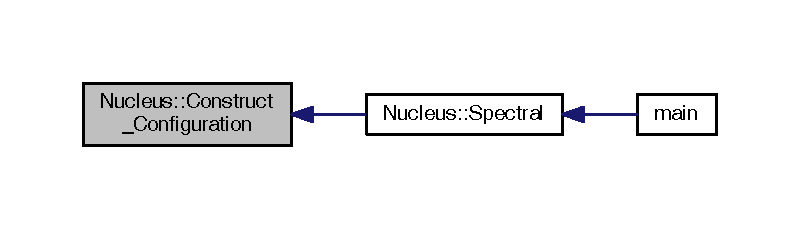
\includegraphics[width=350pt]{class_nucleus_a5f953c3273fccb833c90c929e6c991a2_icgraph}
\end{center}
\end{figure}


\hypertarget{class_nucleus_a5e449f1e876db72824f9466131becac0}{\index{Nucleus@{Nucleus}!Spectral@{Spectral}}
\index{Spectral@{Spectral}!Nucleus@{Nucleus}}
\subsubsection[{Spectral}]{\setlength{\rightskip}{0pt plus 5cm}void Nucleus\-::\-Spectral (
\begin{DoxyParamCaption}
\item[{vec \&}]{J, }
\item[{vec \&}]{Parity}
\end{DoxyParamCaption}
)}}\label{class_nucleus_a5e449f1e876db72824f9466131becac0}


Spectral with angular momentum projection. 


\begin{DoxyParams}{Parameters}
{\em J} & angular momentum \\
\hline
{\em P} & parity \\
\hline
\end{DoxyParams}
\begin{DoxyReturn}{Returns}
Excited energies 
\end{DoxyReturn}


Here is the call graph for this function\-:
\nopagebreak
\begin{figure}[H]
\begin{center}
\leavevmode
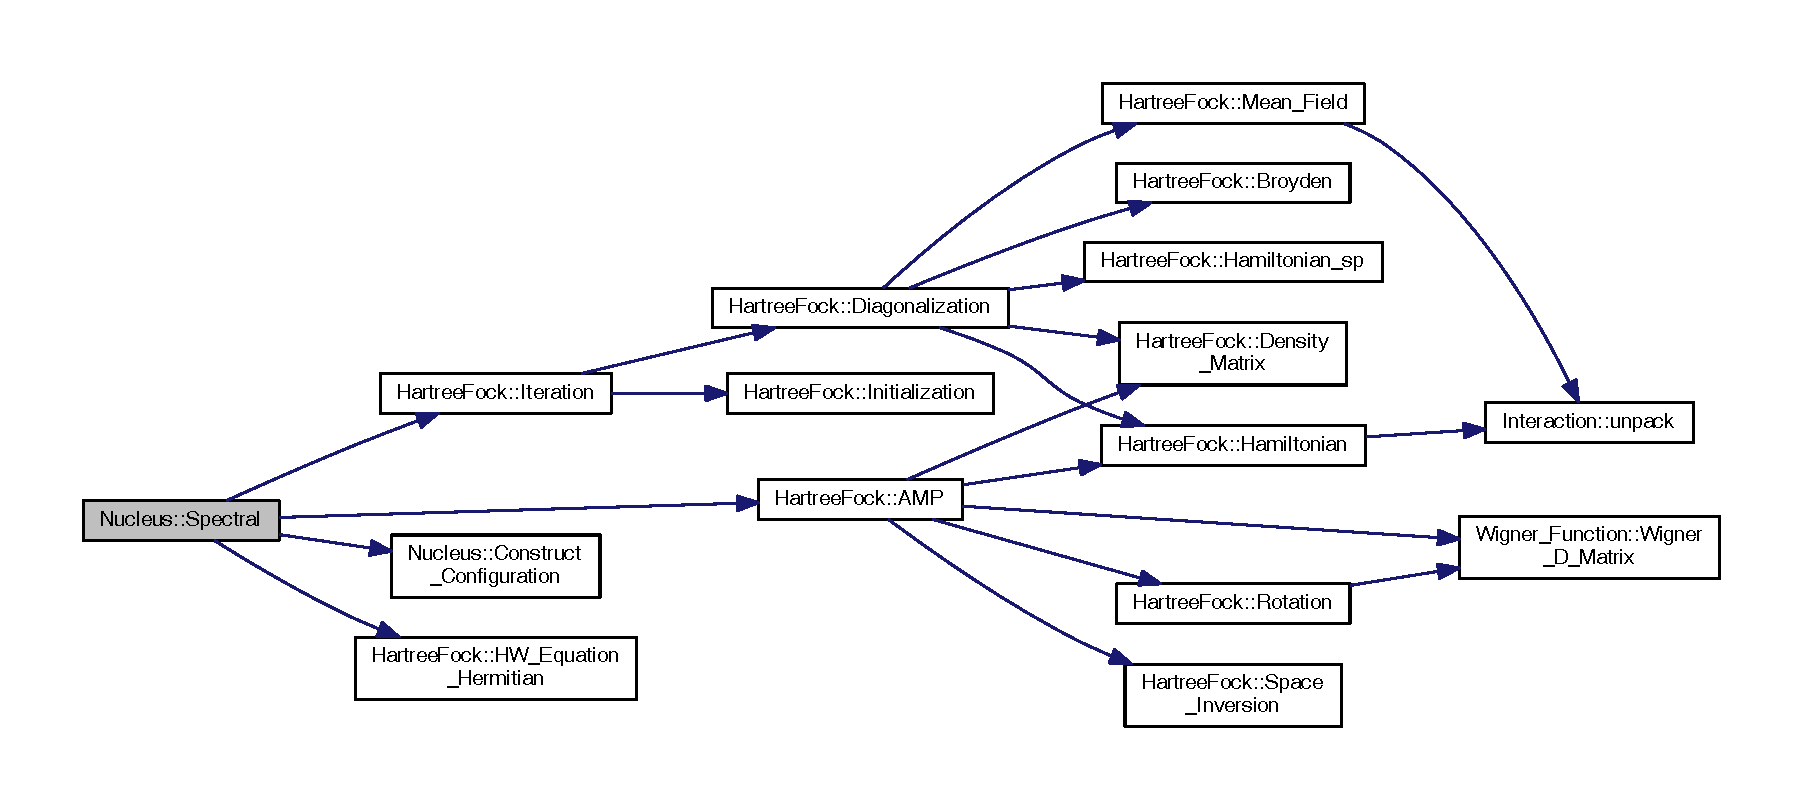
\includegraphics[width=350pt]{class_nucleus_a5e449f1e876db72824f9466131becac0_cgraph}
\end{center}
\end{figure}




Here is the caller graph for this function\-:
\nopagebreak
\begin{figure}[H]
\begin{center}
\leavevmode
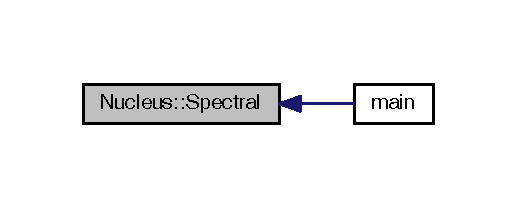
\includegraphics[width=248pt]{class_nucleus_a5e449f1e876db72824f9466131becac0_icgraph}
\end{center}
\end{figure}


\hypertarget{class_nucleus_a2f41a5f6ec0546ec57736d5f0bad6e17}{\index{Nucleus@{Nucleus}!Spectral@{Spectral}}
\index{Spectral@{Spectral}!Nucleus@{Nucleus}}
\subsubsection[{Spectral}]{\setlength{\rightskip}{0pt plus 5cm}void Nucleus\-::\-Spectral (
\begin{DoxyParamCaption}
{}
\end{DoxyParamCaption}
)}}\label{class_nucleus_a2f41a5f6ec0546ec57736d5f0bad6e17}


Spectral with angular momentum projection. 

\begin{DoxyReturn}{Returns}
Excited energies 
\end{DoxyReturn}


Here is the call graph for this function\-:
\nopagebreak
\begin{figure}[H]
\begin{center}
\leavevmode
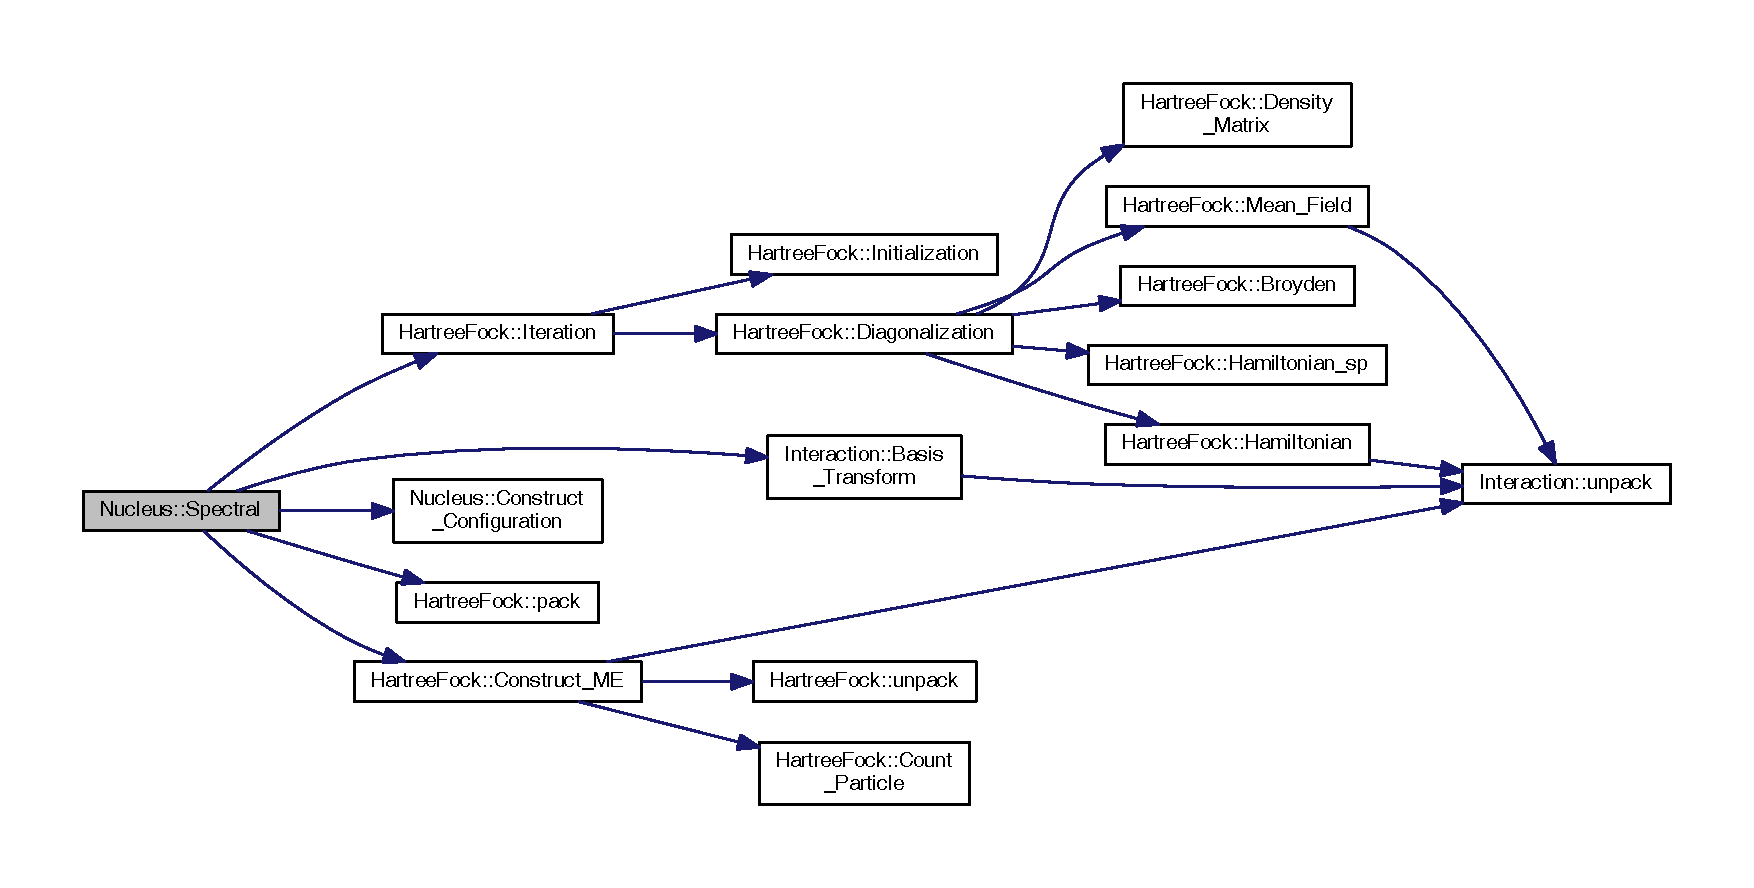
\includegraphics[width=350pt]{class_nucleus_a2f41a5f6ec0546ec57736d5f0bad6e17_cgraph}
\end{center}
\end{figure}




\subsection{Member Data Documentation}
\hypertarget{class_nucleus_a26891e375a90425a013eab9c7176f318}{\index{Nucleus@{Nucleus}!Basis@{Basis}}
\index{Basis@{Basis}!Nucleus@{Nucleus}}
\subsubsection[{Basis}]{\setlength{\rightskip}{0pt plus 5cm}{\bf Hartree\-Fock} Nucleus\-::\-Basis\hspace{0.3cm}{\ttfamily [private]}}}\label{class_nucleus_a26891e375a90425a013eab9c7176f318}
\hypertarget{class_nucleus_a0bca60cd6f52b789fa096d0f5ce2a75e}{\index{Nucleus@{Nucleus}!Configuration@{Configuration}}
\index{Configuration@{Configuration}!Nucleus@{Nucleus}}
\subsubsection[{Configuration}]{\setlength{\rightskip}{0pt plus 5cm}imat Nucleus\-::\-Configuration\mbox{[}{\bf Interaction}$<$ double $>$\-::Iso\-Spin\-\_\-\-Z\mbox{]}\hspace{0.3cm}{\ttfamily [private]}}}\label{class_nucleus_a0bca60cd6f52b789fa096d0f5ce2a75e}


The documentation for this class was generated from the following file\-:\begin{DoxyCompactItemize}
\item 
\hyperlink{main_8cpp}{main.\-cpp}\end{DoxyCompactItemize}

\hypertarget{class_wigner___function}{\section{Wigner\-\_\-\-Function Class Reference}
\label{class_wigner___function}\index{Wigner\-\_\-\-Function@{Wigner\-\_\-\-Function}}
}
\subsection*{Public Member Functions}
\begin{DoxyCompactItemize}
\item 
double \hyperlink{class_wigner___function_a9e5617cceb841b8a82275ac6ef3f6bcb}{Wigner\-\_\-d\-\_\-\-Matrix} (double j, double m1, double m2, double beta)
\item 
cx\-\_\-double \hyperlink{class_wigner___function_a28e07d8d28a1f74ecf63384106444c19}{Wigner\-\_\-\-D\-\_\-\-Matrix} (double j, double m1, double m2, double alpha, double beta, double gamma)
\end{DoxyCompactItemize}


\subsection{Member Function Documentation}
\hypertarget{class_wigner___function_a9e5617cceb841b8a82275ac6ef3f6bcb}{\index{Wigner\-\_\-\-Function@{Wigner\-\_\-\-Function}!Wigner\-\_\-d\-\_\-\-Matrix@{Wigner\-\_\-d\-\_\-\-Matrix}}
\index{Wigner\-\_\-d\-\_\-\-Matrix@{Wigner\-\_\-d\-\_\-\-Matrix}!Wigner_Function@{Wigner\-\_\-\-Function}}
\subsubsection[{Wigner\-\_\-d\-\_\-\-Matrix}]{\setlength{\rightskip}{0pt plus 5cm}double Wigner\-\_\-\-Function\-::\-Wigner\-\_\-d\-\_\-\-Matrix (
\begin{DoxyParamCaption}
\item[{double}]{j, }
\item[{double}]{m1, }
\item[{double}]{m2, }
\item[{double}]{beta}
\end{DoxyParamCaption}
)}}\label{class_wigner___function_a9e5617cceb841b8a82275ac6ef3f6bcb}


Here is the call graph for this function\-:
\nopagebreak
\begin{figure}[H]
\begin{center}
\leavevmode
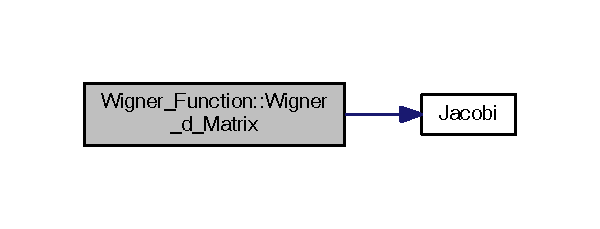
\includegraphics[width=288pt]{class_wigner___function_a9e5617cceb841b8a82275ac6ef3f6bcb_cgraph}
\end{center}
\end{figure}


\hypertarget{class_wigner___function_a28e07d8d28a1f74ecf63384106444c19}{\index{Wigner\-\_\-\-Function@{Wigner\-\_\-\-Function}!Wigner\-\_\-\-D\-\_\-\-Matrix@{Wigner\-\_\-\-D\-\_\-\-Matrix}}
\index{Wigner\-\_\-\-D\-\_\-\-Matrix@{Wigner\-\_\-\-D\-\_\-\-Matrix}!Wigner_Function@{Wigner\-\_\-\-Function}}
\subsubsection[{Wigner\-\_\-\-D\-\_\-\-Matrix}]{\setlength{\rightskip}{0pt plus 5cm}cx\-\_\-double Wigner\-\_\-\-Function\-::\-Wigner\-\_\-\-D\-\_\-\-Matrix (
\begin{DoxyParamCaption}
\item[{double}]{j, }
\item[{double}]{m1, }
\item[{double}]{m2, }
\item[{double}]{alpha, }
\item[{double}]{beta, }
\item[{double}]{gamma}
\end{DoxyParamCaption}
)\hspace{0.3cm}{\ttfamily [inline]}}}\label{class_wigner___function_a28e07d8d28a1f74ecf63384106444c19}


Here is the caller graph for this function\-:
\nopagebreak
\begin{figure}[H]
\begin{center}
\leavevmode
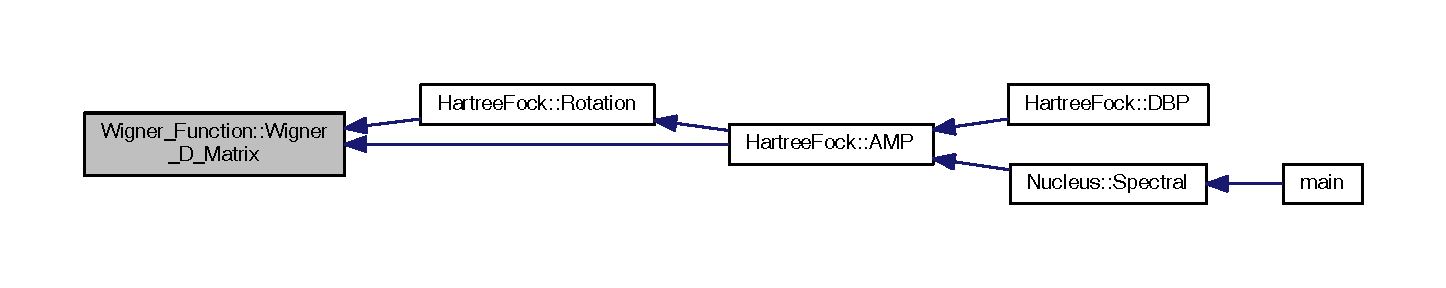
\includegraphics[width=350pt]{class_wigner___function_a28e07d8d28a1f74ecf63384106444c19_icgraph}
\end{center}
\end{figure}




The documentation for this class was generated from the following file\-:\begin{DoxyCompactItemize}
\item 
\hyperlink{main_8cpp}{main.\-cpp}\end{DoxyCompactItemize}

\chapter{File Documentation}
\hypertarget{main_8cpp}{\section{main.\-cpp File Reference}
\label{main_8cpp}\index{main.\-cpp@{main.\-cpp}}
}
{\ttfamily \#include $<$iostream$>$}\\*
{\ttfamily \#include $<$fstream$>$}\\*
{\ttfamily \#include $<$sstream$>$}\\*
{\ttfamily \#include $<$iomanip$>$}\\*
{\ttfamily \#include $<$cmath$>$}\\*
{\ttfamily \#include $<$complex$>$}\\*
{\ttfamily \#include $<$cstdio$>$}\\*
{\ttfamily \#include $<$cstdlib$>$}\\*
{\ttfamily \#include $<$string$>$}\\*
{\ttfamily \#include $<$bitset$>$}\\*
{\ttfamily \#include $<$limits$>$}\\*
{\ttfamily \#include $<$algorithm$>$}\\*
{\ttfamily \#include $<$vector$>$}\\*
{\ttfamily \#include $<$ctime$>$}\\*
{\ttfamily \#include $<$gsl/gsl\-\_\-math.\-h$>$}\\*
{\ttfamily \#include $<$gsl/gsl\-\_\-combination.\-h$>$}\\*
{\ttfamily \#include $<$gsl/gsl\-\_\-complex.\-h$>$}\\*
{\ttfamily \#include $<$gsl/gsl\-\_\-complex\-\_\-math.\-h$>$}\\*
{\ttfamily \#include $<$gsl/gsl\-\_\-block.\-h$>$}\\*
{\ttfamily \#include $<$gsl/gsl\-\_\-vector.\-h$>$}\\*
{\ttfamily \#include $<$gsl/gsl\-\_\-matrix.\-h$>$}\\*
{\ttfamily \#include $<$gsl/gsl\-\_\-multimin.\-h$>$}\\*
{\ttfamily \#include $<$gsl/gsl\-\_\-sf\-\_\-coupling.\-h$>$}\\*
{\ttfamily \#include $<$gsl/gsl\-\_\-blas.\-h$>$}\\*
{\ttfamily \#include $<$gsl/gsl\-\_\-rng.\-h$>$}\\*
{\ttfamily \#include $<$gsl/gsl\-\_\-randist.\-h$>$}\\*
{\ttfamily \#include $<$gsl/gsl\-\_\-eigen.\-h$>$}\\*
{\ttfamily \#include $<$gsl/gsl\-\_\-sort.\-h$>$}\\*
{\ttfamily \#include $<$gsl/gsl\-\_\-sort\-\_\-vector.\-h$>$}\\*
{\ttfamily \#include $<$gsl/gsl\-\_\-sf\-\_\-gamma.\-h$>$}\\*
{\ttfamily \#include $<$gsl/gsl\-\_\-chebyshev.\-h$>$}\\*
{\ttfamily \#include $<$gsl/gsl\-\_\-sf\-\_\-legendre.\-h$>$}\\*
{\ttfamily \#include $<$gsl/gsl\-\_\-sf\-\_\-hyperg.\-h$>$}\\*
{\ttfamily \#include $<$gsl/gsl\-\_\-sf\-\_\-pow\-\_\-int.\-h$>$}\\*
{\ttfamily \#include $<$gsl/gsl\-\_\-linalg.\-h$>$}\\*
{\ttfamily \#include $<$gsl/gsl\-\_\-integration.\-h$>$}\\*
{\ttfamily \#include $<$gsl/gsl\-\_\-fft\-\_\-real.\-h$>$}\\*
{\ttfamily \#include $<$gsl/gsl\-\_\-fft\-\_\-halfcomplex.\-h$>$}\\*
{\ttfamily \#include $<$gsl/gsl\-\_\-bspline.\-h$>$}\\*
{\ttfamily \#include $<$gsl/gsl\-\_\-spline.\-h$>$}\\*
{\ttfamily \#include $<$gsl/gsl\-\_\-errno.\-h$>$}\\*
{\ttfamily \#include $<$gsl/gsl\-\_\-fft\-\_\-complex.\-h$>$}\\*
{\ttfamily \#include $<$gsl/gsl\-\_\-roots.\-h$>$}\\*
{\ttfamily \#include $<$armadillo$>$}\\*
{\ttfamily \#include $<$omp.\-h$>$}\\*
Include dependency graph for main.\-cpp\-:
\nopagebreak
\begin{figure}[H]
\begin{center}
\leavevmode
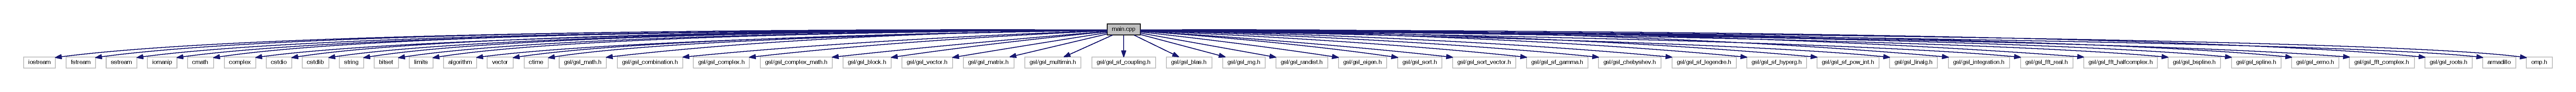
\includegraphics[width=350pt]{main_8cpp__incl}
\end{center}
\end{figure}
\subsection*{Classes}
\begin{DoxyCompactItemize}
\item 
class \hyperlink{class_wigner___function}{Wigner\-\_\-\-Function}
\item 
class \hyperlink{class_j___orbit}{J\-\_\-\-Orbit}
\item 
class \hyperlink{class_m___state}{M\-\_\-\-State}
\item 
struct \hyperlink{struct_coupled___state}{Coupled\-\_\-\-State}
\item 
class \hyperlink{class_interaction}{Interaction$<$ T $>$}
\item 
class \hyperlink{class_hartree_fock}{Hartree\-Fock}
\item 
class \hyperlink{class_nucleus}{Nucleus}
\end{DoxyCompactItemize}
\subsection*{Functions}
\begin{DoxyCompactItemize}
\item 
double \hyperlink{main_8cpp_a15f6d1a273d95f84822a2c49fd2829ac}{Jacobi} (double x, int n, double a, double b)
\item 
int \hyperlink{main_8cpp_a3c04138a5bfe5d72780bb7e82a18e627}{main} (int argc, char $\ast$$\ast$argv)
\end{DoxyCompactItemize}


\subsection{Function Documentation}
\hypertarget{main_8cpp_a15f6d1a273d95f84822a2c49fd2829ac}{\index{main.\-cpp@{main.\-cpp}!Jacobi@{Jacobi}}
\index{Jacobi@{Jacobi}!main.cpp@{main.\-cpp}}
\subsubsection[{Jacobi}]{\setlength{\rightskip}{0pt plus 5cm}double Jacobi (
\begin{DoxyParamCaption}
\item[{double}]{x, }
\item[{int}]{n, }
\item[{double}]{a, }
\item[{double}]{b}
\end{DoxyParamCaption}
)}}\label{main_8cpp_a15f6d1a273d95f84822a2c49fd2829ac}


Here is the caller graph for this function\-:
\nopagebreak
\begin{figure}[H]
\begin{center}
\leavevmode
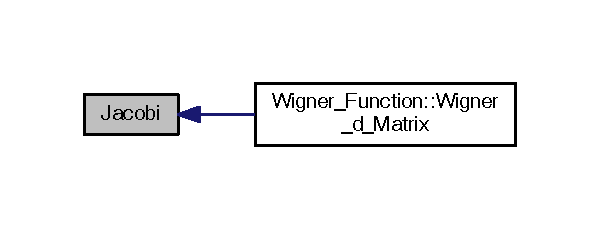
\includegraphics[width=288pt]{main_8cpp_a15f6d1a273d95f84822a2c49fd2829ac_icgraph}
\end{center}
\end{figure}


\hypertarget{main_8cpp_a3c04138a5bfe5d72780bb7e82a18e627}{\index{main.\-cpp@{main.\-cpp}!main@{main}}
\index{main@{main}!main.cpp@{main.\-cpp}}
\subsubsection[{main}]{\setlength{\rightskip}{0pt plus 5cm}int main (
\begin{DoxyParamCaption}
\item[{int}]{argc, }
\item[{char $\ast$$\ast$}]{argv}
\end{DoxyParamCaption}
)}}\label{main_8cpp_a3c04138a5bfe5d72780bb7e82a18e627}
\hyperlink{class_nucleus}{Nucleus} S\-D(Z,A,\char`\"{}sd.\-sps\char`\"{},\char`\"{}usdb.\-int\char`\"{});

S\-D.\-Spectral(\-J,\-P); 

Here is the call graph for this function\-:
\nopagebreak
\begin{figure}[H]
\begin{center}
\leavevmode
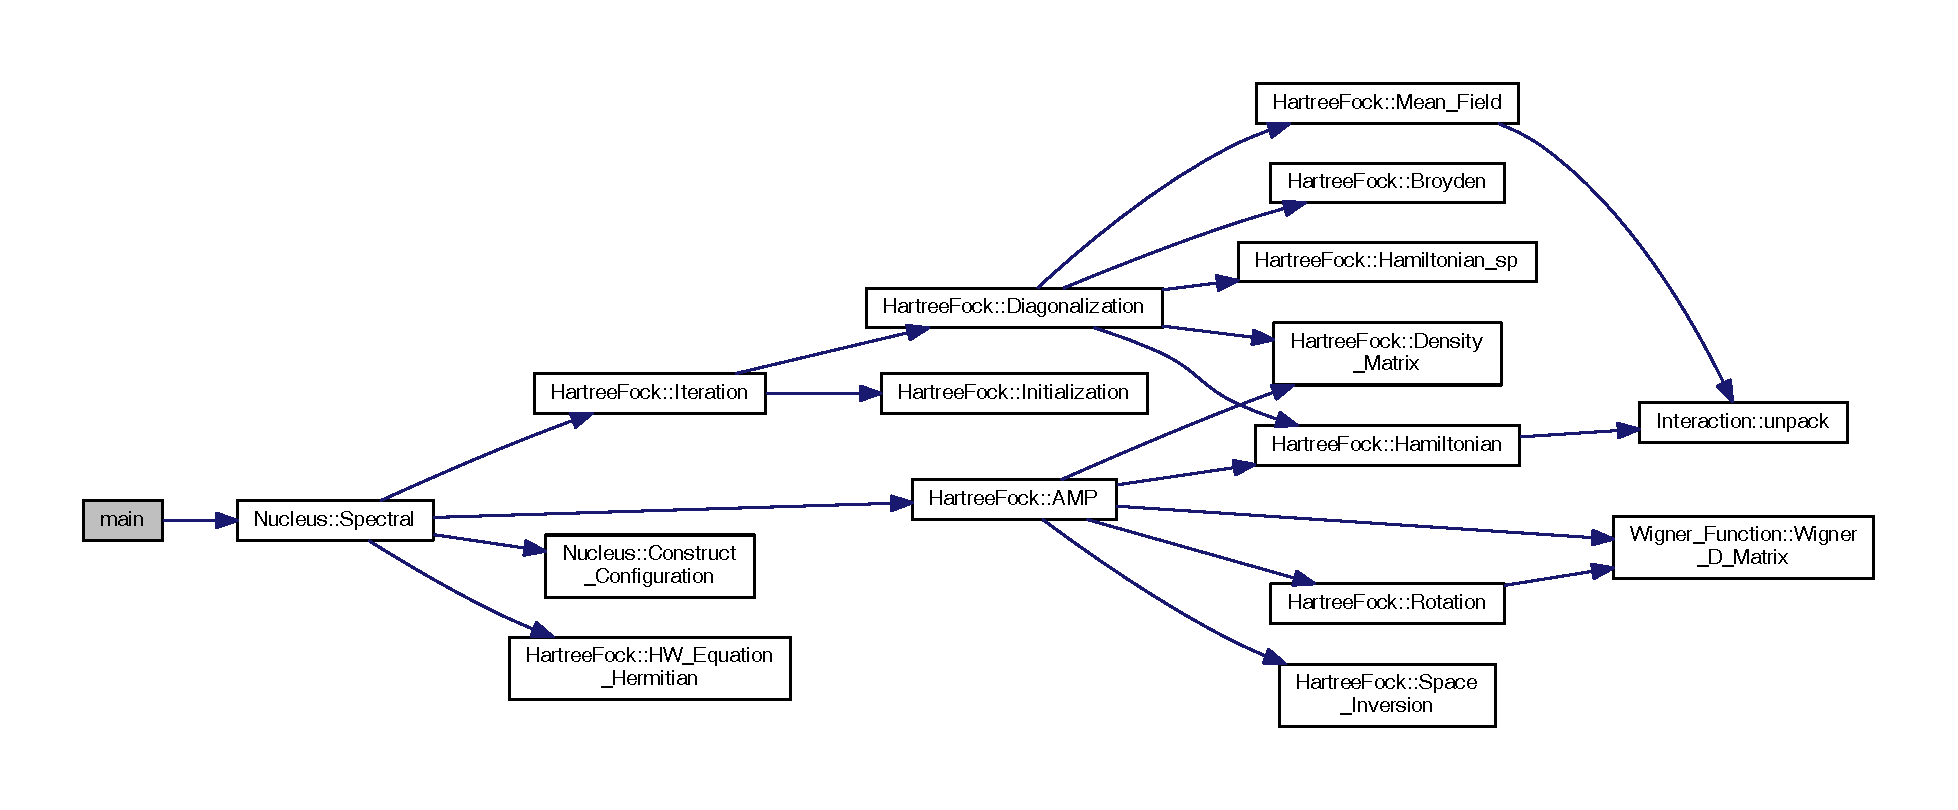
\includegraphics[width=350pt]{main_8cpp_a3c04138a5bfe5d72780bb7e82a18e627_cgraph}
\end{center}
\end{figure}



%--- End generated contents ---

% Index
\newpage
\phantomsection
\addcontentsline{toc}{part}{Index}
\printindex

\end{document}
